%%%%%%%%%%%%%%%%%%%%%%%%%%%%%%%%%%%%%%%%%%%%%%%%%%%%%%%%%%%%%%%%%%%%%%
% Lớp 11 | Hàm số lượng giác và phương trình lượng giác | Giá trị lượng giác của một góc lượng giác
% Dạng 1D1?2-3: Biến đổi, rút gọn biểu thức lượng giác; chứng minh đẳng thức lượng giác
% Số câu: 112  (sinh tự động bởi tach_cau.py; từ nay thầy sửa trực tiếp file này)
%%%%%%%%%%%%%%%%%%%%%%%%%%%%%%%%%%%%%%%%%%%%%%%%%%%%%%%%%%%%%%%%%%%%%%

%%%%%%%%%%%%%%%% TRẮC NGHIỆM 4 PHƯƠNG ÁN %%%%%%%%%%%%%%%%

% nguồn: Ok_Toan11_TracNghiem_Lan2
\begin{ex}%[1D1N2-3]%[ma:349c267a]
	Tính $ L=\tan20^\circ \cdot  \tan45^\circ\cdot \tan70^\circ$.
	\choice 
		 {$ 0$}
		{\True $  1$}
		{$-1$} 
		{$ 2$} 
	 \loigiai{ Ta có
		\allowdisplaybreaks\begin{eqnarray*}
		L&=&\tan20^\circ \cdot \tan45^\circ\cdot  \tan70^\circ\\
		&=& \left(\tan 20^\circ\tan 70^\circ\right)\tan 45^\circ\\ 
		 &=& \left(\tan 20^\circ \cot 20^\circ \right)\tan 45^\circ\\
		 &=&1.
\end{eqnarray*}}
\end{ex}

% nguồn: Ok_Toan11_TracNghiem_Lan2
\begin{ex}%[1D1N2-3]%[ma:d89bd8df]
	Đơn giản biểu thức $P=\left(\dfrac{\sin \alpha+\tan \alpha}{\cos \alpha+1} \right)^2+1$. 
	\choice 
		{$P=2$} 
		{$P=1+\tan  \alpha$}
		 {\True $P=\dfrac{1}{\cos ^2\alpha}$}
		{$P=\dfrac{1}{\sin  ^2\alpha}$}
	\loigiai{ 
		Ta có 
		\[\dfrac{\sin \alpha+\tan \alpha}{\cos \alpha+1}=\dfrac{\sin \alpha \left(1+\dfrac{1}{\cos \alpha} \right)}{\cos \alpha+1}=\dfrac{\sin \alpha \left(\dfrac{\cos \alpha+1}{\cos \alpha} \right)}{\cos  \alpha+1}=\dfrac{\sin \alpha}{\cos \alpha}=\tan \alpha.\]
		Suy  ra $P=\tan ^2\alpha+1=\dfrac{1}{\cos ^2\alpha}$.
	 }
\end{ex}

% nguồn: Ok_Toan11_TracNghiem_Lan2
\begin{ex}%[1D1N2-3]%[ma:3679d60e]
	Rút gọn biểu thức $M=\left(\sin ^4x+\cos ^4x-1\right)\left(\tan  ^2x+\cot ^2x+2\right)$.
	\choice 
		{$M=-4$} 
		{\True  $M=-2$}
		 {$M=2$}
		 {$M=4$}
	 \loigiai{
		 Ta có
		\begin{align*}
			M&=\left(1-2\sin ^2x\cdot \cos ^2x-1\right)\left(\dfrac{\sin  ^2x}{\cos ^2x}+\dfrac{\cos ^2x}{\sin ^2x}+2\right)\\
			 &=\left(-2\sin ^2x\cdot \cos ^2x\right)\left(\dfrac{\sin ^4x+\cos ^4x+2\sin ^2x\cdot \cos ^2x}{\sin ^2x\cos ^2x} \right)\\
			 &=\left(-2\right)\cdot \left(\sin ^2x+\cos ^2x\right)^2=-2.
		\end{align*}
	 }
\end{ex}

% nguồn: Ok_Toan11_TracNghiem_Lan2
\begin{ex}%[1D1N2-3]%[ma:0c2179d2]
	Đơn giản biểu thức  $P=\dfrac{2\cos ^2x-1}{\sin x+\cos x}$.
	\choice 
		{$P=\cos x+\sin  x$}
		 {\True $P=\cos x-\sin x$}
		{$P=\cos 2x-\sin  2x$}
		 {$P=\cos 2x+\sin 2x$}
	\loigiai{ 
		Ta có $P=\dfrac{2\cos ^2x-\left(\sin ^2x+\cos  ^2x\right)}{\sin x+\cos x}=\dfrac{\cos ^2x-\sin ^2x}{\sin x+\cos x}=\cos x-\sin x$.
	} 
\end{ex}

% nguồn: Ok_Toan11_TracNghiem_Lan2
\begin{ex}%[1D1N2-3]%[ma:a1932996]
	Đơn giản biểu thức $P=\dfrac{\cot ^2x-\cos^2x}{\cot  ^2x}+\dfrac{\sin x \cos x}{\cot x}$.
	\choice 
		 {\True $P=1$}
		{$P=-1$} 
		 {$P=\dfrac{1}{2}$}
		 {$P=-\dfrac{1}{2}$}
	\loigiai{ 
		Ta  có
		\begin{itemize}
			\item $\dfrac{\cot  ^2x-\cos^2x}{\cot ^2x}=1-\dfrac{\cos ^2x}{\cot ^2x}=1-\cos ^2x\cdot \dfrac{\sin ^2x}{\cos ^2x}=1-\sin ^2x$.
			\item $\dfrac{\sin x\cdot \cos  x}{\cot x}=\sin x\cdot \cos x\cdot \dfrac{\sin x}{\cos x}=\sin ^2x$.
		\end{itemize}
		Suy ra $P=1-\sin ^2x+\sin  ^2x=1$.
	} 
\end{ex}

% nguồn: Ok_Toan11_TracNghiem_Lan2
\begin{ex}%[1D1N2-3]%[ma:1c42c39a]
	Rút  gọn biểu thức $M=\tan ^2x-\sin ^2x$.
	\choice 
		{$M=\tan ^2x$} 
		{$M=\sin ^2x$} 
		{\True  $M=\tan ^2x\cdot \sin ^2x$}
		 {$M=1$}
	 \loigiai{
		Ta có $M=\tan ^2x-\sin ^2x=\dfrac{\sin  ^2x}{\cos ^2x}-\sin ^2x=\sin ^2x\left(\dfrac{1}{\cos ^2x}-1\right)=\sin ^2x\cdot \tan ^2x$.
	} 
\end{ex}

% nguồn: Ok_Toan11_TracNghiem_Lan2
\begin{ex}%[1D1N2-3]%[ma:f12b210d]
	Rút gọn  biểu thức $M=\sin ^2\alpha \tan ^2\alpha+4\sin ^2\alpha-\tan ^2\alpha+3\cos ^2\alpha$.
	 \choice
		{$M=1+\sin ^2\alpha$} 
		{$M=\sin  \alpha$}
		{$M=2\sin  \alpha$}
		 {\True $M=3$}
	\loigiai{ 
		Ta có 
		\begin{align*}
			 M&=\tan ^2\alpha \left(\sin ^2\alpha-1\right)+4\sin ^2\alpha+3\cos ^2\alpha\\
			&=\tan ^2\alpha  \left(-\cos ^2\alpha \right)+4\sin ^2\alpha+3\cos ^2\alpha\\
			&=-\sin  ^2\alpha+4\sin ^2\alpha+3\cos ^2\alpha\\
			&=3\left(\sin  ^2\alpha+\cos ^2\alpha \right)=3.
		\end{align*}
	} 
\end{ex}

% nguồn: Ok_Toan11_TracNghiem_Lan2
\begin{ex}%[1D1N2-3]%[ma:bf781204]
	Rút gọn biểu thức $M=\sin  ^6x+\cos ^6x$.
	 \choice
		{$M=1+3\sin ^2x\cos  ^2x$}
		{$M=1-3\sin ^2x$} 
		{$M=1-\dfrac{3}{2}  \sin ^22x$}
		{\True $M=1-\dfrac{3}{4}  \sin ^22x$}
	\loigiai{ 
		Ta  có
		\begin{align*}
			M&=\sin  ^6x+\cos ^6x=\left(\sin ^2x\right)^3+\left(\cos ^2x\right)^3\\
			&=\left(\sin ^2x+\cos ^2x\right)^3-3\sin  ^2x\cos ^2x\left(\sin ^2x+\cos ^2x\right)\\
			&=1-3\sin  ^2x\cos ^2x=1-\dfrac{3}{4} \sin ^22x.
		\end{align*}
	 }
\end{ex}

% nguồn: Ok_Toan11_TracNghiem_Lan2
\begin{ex}%[1D1N2-3]%[ma:510cae04]
	 Đơn giản biểu thức $P=\dfrac{1-\sin ^2\alpha \cos ^2\alpha}{\cos ^2\alpha}-\cos ^2\alpha$.
	\choice 
		{\True  $P=\tan ^2\alpha$}
		{$P=1$} 
		{$P=-\cos ^2\alpha$} 
		{$P=\cot ^2\alpha$} 
	\loigiai{ 
		\begin{align*}
			P&=\dfrac{1-\sin ^2\alpha \cos ^2\alpha-\cos ^4\alpha}{\cos  ^2\alpha}\\
			&=\dfrac{1-\cos ^2\alpha \left(\sin ^2\alpha+\cos  ^2\alpha \right)}{\cos ^2\alpha}\\
			&=\dfrac{1-\cos ^2\alpha}{\cos ^2\alpha}=\dfrac{\sin ^2\alpha}{\cos  ^2\alpha}=\tan ^2\alpha.
		\end{align*}
	 }
\end{ex}

% nguồn: Ok_Toan11_TracNghiem_Lan2
\begin{ex}%[1D1N2-3]%[ma:2f3f57c4]
	Rút gọn biểu thức $M=\cot  ^2x-\cos ^2x$.
	\choice 
		 {$M=\cot ^2x$}
		 {$M=\cos ^2x$}
		{$M=1$} 
		{\True $M=\cot  ^2x\cdot \cos ^2x$}
	\loigiai{ 
		Ta có $M=\cot ^2x-\cos  ^2x=\dfrac{\cos ^2x}{\sin ^2x}-\cos ^2x=\cos ^2x\left(\dfrac{1}{\sin ^2x}-1\right)=\cos ^2x\cdot \cot ^2x$.
	 }
\end{ex}

% nguồn: Ok_Toan11_TracNghiem_Lan2
\begin{ex}%[1D1N2-3]%[ma:f08a6298]
	Đơn giản  biểu thức $P=\tan \alpha \left(\dfrac{1+\cos ^2\alpha}{\sin \alpha}-\sin \alpha \right)$.
	\choice 
		{$P=2$} 
		 {\True $P=2\cos \alpha$}
		 {$P=2\tan \alpha$}
		{$P=2\sin  \alpha$}
	\loigiai{ 
		Ta  có
		\begin{align*}
			P&=\tan \alpha \left(\dfrac{1+\cos ^2\alpha}{\sin \alpha}-\sin \alpha  \right)=\dfrac{\sin \alpha}{\cos \alpha} \left(\dfrac{1}{\sin \alpha}+\dfrac{\cos ^2\alpha}{\sin \alpha}-\sin \alpha \right)=\dfrac{1}{\cos \alpha}+\cos \alpha-\dfrac{\sin ^2\alpha}{\cos \alpha}\\
			&=\dfrac{1+\cos ^2\alpha-\sin ^2\alpha}{\cos  \alpha}=\dfrac{\left(1-\sin ^2\alpha \right)+\cos ^2\alpha}{\cos \alpha}=\dfrac{2\cos ^2\alpha}{\cos \alpha}=2\cos \alpha.
		\end{align*}
	} 
\end{ex}

% nguồn: Ok_Toan11_TracNghiem_Lan2
\begin{ex}%[1D1N2-3]%[ma:984549d9]
	Tính  $ A=\sin{390^\circ}-2\sin{1140^\circ}+3\cos{1845^\circ}$
	\choice 
		{\True $\dfrac{1}{2}\left(1+3\sqrt{2}-2\sqrt{3}\right)$} 
		 {$\dfrac{1}{2}\left(1-3\sqrt{2}-2\sqrt{3}\right)$}
		{$\dfrac{1}{2}\left(1+2\sqrt{3}-3\sqrt{2}\right)$} 
		 {$\dfrac{1}{2}\left(1+2\sqrt{3}+3\sqrt{2}\right)$}
	\loigiai{Ta  có
		\allowdisplaybreaks\begin{eqnarray*}
		A&=&\sin 390^\circ-2\sin 1140^\circ +3\cos 1845^\circ \\ 
		&=&\sin\left(2\cdot 180^\circ+30^\circ\right)-2\sin\left(6\cdot  180^\circ+60^\circ\right)+3\cos\left(10\cdot 180^\circ+45^\circ\right)\\
		 &=& \sin 30^\circ -2\sin 60^\circ+3\cos45^\circ\\
		 &=& \dfrac{1}{2}-2\cdot \dfrac{\sqrt{3}}{2}+3\cdot\dfrac{\sqrt{2}}{2}\\
		 &=&\dfrac{1}{2}\left(1-2\sqrt{3}+3\sqrt{2}\right).
	\end{eqnarray*}
} 
\end{ex}

% nguồn: Ok_Toan11_TracNghiem_Lan2
\begin{ex}%[1D1N2-3]%[ma:3cc2eef3]
	Đơn giản biểu thức  $P=\dfrac{1-\cos \alpha}{\sin ^2\alpha}-\dfrac{1}{1+\cos \alpha}$.
	\choice 
		 {$P=-\dfrac{2\cos \alpha}{\sin ^2\alpha}$}
		 {$P=\dfrac{2}{\sin ^2\alpha}$}
		 {$P=\dfrac{2}{1+\cos \alpha}$}
		 {\True $P=0$}
	 \loigiai{
		Ta có 
		\begin{align*}
			P&=\dfrac{1-\cos \alpha}{\sin  ^2\alpha}-\dfrac{1}{1+\cos \alpha}\\
			 &=\dfrac{1-\cos \alpha}{1-\cos ^2\alpha}-\dfrac{1}{1+\cos \alpha}\\
			&=\dfrac{1-\cos \alpha}{\left(1-\cos \alpha  \right)\left(1+\cos \alpha \right)}-\dfrac{1}{1+\cos \alpha}\\
			&=\dfrac{1}{1+\cos \alpha}-\dfrac{1}{1+\cos \alpha}=0. 
		\end{align*}
	 }
\end{ex}

% nguồn: Ok_Toan11_TracNghiem_Lan2
\begin{ex}%[1D1N2-3]%[ma:87bc3cd3]
	Đơn giản biểu thức $P=\dfrac{1+\sin ^2\alpha}{1-\sin ^2\alpha}$. 
	\choice 
		{\True $P=1+2\tan  ^2\alpha$}
		{$P=1-2\tan ^2\alpha$} 
		{$P=-1+2\tan ^2\alpha$} 
		 {$P=-1-2\tan ^2\alpha$}
	 \loigiai{
		 Ta có $P=\dfrac{1+\sin ^2\alpha}{1-\sin ^2\alpha}=\dfrac{1+\sin ^2\alpha}{\cos^2\alpha}=\dfrac{1}{\cos^2\alpha}+\tan ^2\alpha=1+2\tan ^2\alpha$.
	} 
\end{ex}

% nguồn: Ok_Toan11_TracNghiem_Lan2
\begin{ex}%[1D1N2-3]%[ma:39813761]
	Rút gọn biểu thức $M=\left(1-\sin ^2x\right)\cot ^2x+\left(1-\cot ^2x\right)$. 
	\choice 
		{\True $M=\sin ^2x$} 
		{$M=\cos  ^2x$}
		{$M=\sin  ^2x$}
		 {$M=\cos ^2x$}
	\loigiai{ 
		Ta biến  đổi $M=\left(\cot ^2x-\cos ^2x\right)+\left(1-\cot ^2x\right)=1-\cos ^2x=\sin ^2x$.
	 }
\end{ex}

% nguồn: Ok_Toan11_TracNghiem_Lan2
\begin{ex}%[1D1N2-3]%[ma:fed7348e]
	 Biết $\tan x=2$, giá trị của biểu thức $M=\dfrac{3\sin x-2\cos x}{5\cos x+7\sin x}$ bằng
	 \choice
		{$\dfrac{4}{9}$} 
		{$-\dfrac{4}{9}$} 
		{\True $\dfrac{4}{19}$} 
		{$-\dfrac{4}{19}$} 
	\loigiai{ 
		Ta có $\tan x=2\Leftrightarrow \dfrac{\sin x}{\cos x}=2\Leftrightarrow \sin x=2\cos x$ thay $\sin  x=2\cos x$ vào $M$
		\[M=\dfrac{3\cdot 2\cos  x-2\cos x}{5\cos x+7\cdot 2\cos x}=\dfrac{4\cos x}{19\cos x}=\dfrac{4}{19}.\]
	 }
\end{ex}

% nguồn: Ok_Toan11_TracNghiem_Lan2
\begin{ex}%[1D1N2-3]%[ma:6f197c26]
	Cho  $\tan \alpha=\dfrac{1}{2}$. Giá trị của biểu thức $P=\dfrac{\sin \alpha}{2\sin ^3\alpha+3\cos ^3\alpha}$ là
	 \choice
		{\True $\dfrac{5}{26}$} 
		 {$\dfrac{1}{3}$}
		{$-\dfrac{5}{26}$} 
		{$-\dfrac{1}{3}$} 
	\loigiai{ 
		\[P=\dfrac{\sin \alpha}{2\sin ^3\alpha+3\cos  ^3\alpha}=\dfrac{\sin \alpha \left(\sin ^2\alpha+\cos^2\alpha \right)}{2\sin ^3\alpha+3\cos ^3\alpha}=\dfrac{\tan ^3\alpha+\tan \alpha}{2\tan ^3\alpha+3}=\dfrac{5}{26}.\]
	} 
\end{ex}

% nguồn: Ok_TracNghiemLop11_Lan1
\begin{ex}%[1D1N2-3]%[ma:a7a887ed]
	Giá trị biểu thức $C=\cos \dfrac{\pi }{6}+\sin \dfrac{\pi }{2}+\tan \pi +\cot \dfrac{\pi  }{4}$ bằng
	\choice 
		{$C=\dfrac{4-\sqrt{3}}{2}$} 
		{$C=\dfrac{6+\sqrt{3}}{2}$} 
		{\True $C=\dfrac{4+\sqrt{3}}{2}$} 
		 {$C\approx 74{,}03$}
	\loigiai{ 
	 Ta có $C=\cos \dfrac{\pi}{6}+\sin \dfrac{\pi}{2}+\tan \pi +\cot \dfrac{\pi }{4}=\dfrac{\sqrt{3}}{2}+1+0+1=\dfrac{4+\sqrt{3}}{2}$.}
\end{ex}

% nguồn: Ok_TracNghiemLop11_Lan1
\begin{ex}%[1D1N2-3]%[ma:343ab016]
	Cho $\tan \alpha =3$, giá trị của biểu thức $M=\dfrac{2\sin \alpha -5\cos \alpha  }{3\sin \alpha +\cos \alpha }$ bằng
	\choice 
		{\True  $\dfrac{1}{10}$}
		{$0$} 
		{$-\dfrac{13}{6}$} 
		 {$-\dfrac{1}{10}$}
	\loigiai{ 
		Đề cho $\tan \alpha =3$ nên $\cos\alpha  \ne 0$.\\
	Chia tử và mẫu cho  $\cos\alpha $ ta được $M=\dfrac{2\tan \alpha -5}{3\tan \alpha +1}=\dfrac{2\cdot 3-5}{3\cdot 3+1}=\dfrac{1}{10}$.}
\end{ex}

% nguồn: Ok_Toan11_TracNghiem_Lan2
\begin{ex}%[1D1H2-3]%[ma:b52672bb]
	Rút gọn biểu thức $ D=\cos^2x\cdot \cot^2 x+3\cos^2x-\cot^2x+2\sin^2x$ ta được 
	\choice 
		 {\True $D=2$}
		{$D=-2$} 
		{$D=3$} 
		{$D=-3$} 
	\loigiai{ 
		 Ta có
		\allowdisplaybreaks\begin{eqnarray*}
		D&=&\cos^2x\cdot  \cot^2 x+3\cos^2x-\cot^2x+2\sin^2x\\
		&=&\cot^2x\left(\cos^2x-1\right)+2\left(\sin^2x+\cos^2x\right)+\cos^2x\\ 
		&=& \cot^2x\left(-\sin^2x\right) +2+\cos^2x\\ 
		&=&-\cos^2x+2+\cos^2x\\ 
		&=&2. 
	\end{eqnarray*}
} 
\end{ex}

% nguồn: Ok_Toan11_TracNghiem_Lan2
\begin{ex}%[1D1H2-3]%[ma:42b5efed]
	 Tính $ G=\cos^2\dfrac{\pi}{6}+\cos^2\dfrac{2\pi}{6}+...+\cos^2\dfrac{5\pi}{6}+\cos^2\pi$
	\choice 
		 {$ 0$}
		{$  1$}
		{$ 2$} 
		{\True $  3$}
	\loigiai{ Ta có 
		\allowdisplaybreaks\begin{eqnarray*}
		 G&=&\cos^2\dfrac{\pi}{6}+\cos^2\dfrac{2\pi}{6}+\ldots +\cos^2\dfrac{5\pi}{6}+\cos^2\pi\\
		&=&  \cos^2\dfrac{\pi}{6}+\cos^2\dfrac{\pi}{3}+\cos^2\dfrac{\pi}{2}+\cos^2\dfrac{2\pi}{3}+\cos^2\dfrac{5\pi}{6}+\cos^2\pi.\\
		&=& \cos^2\dfrac{\pi}{6}+\sin^2\dfrac{\pi}{6}+\cos^2\dfrac{\pi}{2}+\cos^2\dfrac{2\pi}{3}+\sin^2\dfrac{2\pi}{3}+\cos^2\pi\\ 
		 &=& 3.
	\end{eqnarray*}
 }
\end{ex}

% nguồn: Ok_Toan11_TracNghiem_Lan2
\begin{ex}%[1D1H2-3]%[ma:919fbafc]
	Rút gọn biểu thức  $M=\left(\sin x+\cos x\right)^2+\left(\sin x-\cos x\right)^2$.
	\choice 
		 {$M=1$}
		 {\True $M=2$}
		 {$M=4$}
		{$M=4\sin  x\cdot \cos x$}
	 \loigiai{
		Ta có \begin{itemize}
		 \item $\left(\sin x+\cos x\right)^2=\sin ^2x+\cos ^2x+2\sin x\cdot \cos x=1+2\sin x\cdot \cos x$.
		\item $\left(\sin x-\cos x\right)^2=\sin  ^2x+\cos ^2x-2\sin x\cdot \cos x=1-2\sin x\cdot \cos x$.
	\end{itemize}
	Suy ra $M=2$. 
} 
\end{ex}

% nguồn: Ok_Toan11_TracNghiem_Lan2
\begin{ex}%[1D1H2-3]%[ma:46060eb9]
	Cho $\cos \alpha=-\dfrac{4}{5}$, với $\dfrac{\pi}{2} < \alpha < \pi$. Tính giá trị  của biểu thức $M=10\sin \alpha+5\cos \alpha$.
	\choice 
		{$-10$} 
		 {\True $2$}
		 {$1$}
		{$\dfrac{1}{4}$} 
	 \loigiai{
		Ta có $\sin ^2\alpha=1-\cos ^2\alpha=1-\left(-\dfrac{4}{5} \right)^2=\dfrac{9}{25}  \Rightarrow \sin \alpha=\pm \dfrac{3}{5}$.\\
		Vì $\dfrac{\pi}{2} < \alpha < \pi$ nên  $\sin \alpha=\dfrac{3}{5}$.\\
		 $M=10\sin \alpha+5\cos \alpha=10\cdot\dfrac{3}{5}+5\cdot\left(-\dfrac{4}{5} \right)=2$.
	} 
\end{ex}

% nguồn: Ok_Toan11_TracNghiem_Lan2
\begin{ex}%[1D1H2-3]%[ma:86e04b0c]
	Nếu $\tan \alpha+\cot \alpha=2$  thì $\tan^2\alpha+\cot^2\alpha$ bằng bao nhiêu?
	\choice 
		 {$1$}
		{$4$} 
		 {\True $2$}
		 {$3$}
	 \loigiai{
		Ta  có
		\allowdisplaybreaks 
		\begin{eqnarray*}
			&\tan \alpha+\cot \alpha=2 &\Rightarrow \left(\tan \alpha+\cot \alpha \right)^2=4  \\
			&& \Leftrightarrow \tan  ^2\alpha+\cot ^2\alpha+2\tan \alpha\cdot\cot \alpha=4\\
			 && \Leftrightarrow \tan ^2\alpha+\cot ^2\alpha=2.
		\end{eqnarray*}
	} 
\end{ex}

% nguồn: Ok_Toan11_TracNghiem_Lan2
\begin{ex}%[1D1H2-3]%[ma:780daa00]
	Rút gọn biểu thức $ B=\dfrac{\cos^2x-\sin^2y}{\sin^2x \cdot \sin^2y}-\cot^2x\cdot \cot^2y$ (với điều kiện biểu thức có nghĩa),  ta được
	 \choice
		{$  2$}
		 {$-2$}
		 {$ 1$}
		 {\True $-1$}
	 \loigiai{
		 Ta có
		\allowdisplaybreaks\begin{eqnarray*}
		B&=&\dfrac{\cos^2x-\sin^2y}{\sin^2x\cdot  \sin^2y}-\cot^2x\cdot \cot^2y\\
		 &=&\dfrac{\cos^2x-\sin^2y-\cos^2x\cdot \cos^2 y}{\sin^2x\cdot \sin^2y}\\
		&=&\dfrac{\cos^2x\left(1-\cos^2y\right)-\sin^2y}{\sin^2x\cdot  \sin^2y}\\
		 &=&\dfrac{\cos^2x\cdot \sin^2 y-\sin^2y}{\sin^2x\cdot \sin^2y}\\
		&=&\dfrac{\sin^2y\left(\cos^2x-1\right)}{\sin^2x\cdot \sin^2  y}\\
		&=&\dfrac{-\sin^2x\cdot \sin^2y}{\sin^2x \cdot \sin^2y}\\ 
		 &=&-1.
	\end{eqnarray*}
} 
\end{ex}

% nguồn: Ok_Toan11_TracNghiem_Lan2
\begin{ex}%[1D1H2-3]%[ma:5d429c3a]
	Biểu thức rút gọn của $A=\dfrac{\tan ^2a-\sin ^2a}{\cot ^2a-\cos ^2a}$ bằng 
	 \choice
		 {\True $\tan ^6a$}
		{$\cos  ^6a$}
		 {$\tan ^4a$}
		{$\sin  ^6a$}
	 \loigiai{
		Ta có 
		 \[
		A=\dfrac{\tan^2 a-\sin^2 a}{\cot^2 a-\cos^2 a} \Leftrightarrow  A=\dfrac{\sin^2 a\left(\dfrac{1}{\cos^2 a}-1\right)}{\cos^2\left(\dfrac{1}{\sin^2 a}-1\right)}=\dfrac{\tan^2 a \cdot \tan^2 a}{\cot^2 a}=\tan^6 a.
		 \]
	} 
\end{ex}

% nguồn: Ok_Toan11_TracNghiem_Lan2
\begin{ex}%[1D1H2-3]%[ma:b13338f8]
	Đơn giản biểu thức $P=\dfrac{\left(\sin \alpha+\cos \alpha \right)^2-1}{\cot  \alpha-\sin \alpha \cos\alpha}$.
	\choice 
		{\True $P=2\tan  ^2\alpha$}
		{$P=\dfrac{\sin  \alpha}{\cos ^3\alpha}$}
		 {$P=2\cot ^2\alpha$}
		 {$P=\dfrac{2}{\cos ^2\alpha}$}
	 \loigiai{
		Ta có 
		\begin{align*}
			P&=\dfrac{\left(\sin \alpha+\cos  \alpha \right)^2-1}{\cot \alpha-\sin \alpha \cos \alpha}\\
			 &=\dfrac{\sin ^2\alpha+2\sin \alpha\cdot \cos \alpha+\cos ^2\alpha-1}{\cos \alpha\cdot \left(\dfrac{1}{\sin \alpha}-\sin \alpha \right)}\\
			&=\dfrac{1+2\sin \alpha\cdot \cos \alpha-1}{\cos \alpha\cdot \dfrac{1-\sin ^2\alpha}{\sin  \alpha}}\\
			&=\dfrac{2\sin \alpha\cdot \cos  \alpha}{\dfrac{\cos ^3\alpha}{\sin \alpha}}\\
			&=\dfrac{2\sin ^2\alpha}{\cos ^2\alpha}=2\tan ^2\alpha. 
		\end{align*}
	 }
\end{ex}

% nguồn: Ok_Toan11_TracNghiem_Lan2
\begin{ex}%[1D1H2-3]%[ma:6c601b6f]
	Có bao nhiêu đẳng thức đúng trong  các đẳng thức sau đây?
	\begin{listEX}[2]
		\item  $\cos ^2\alpha=\dfrac{1}{\tan ^2\alpha+1}$.
		\item $\sqrt{2} \cos \left(\alpha+\dfrac{\pi}{4}\right)=\cos  \alpha+\sin \alpha$.
		\item $\sin \left(\alpha-\dfrac{\pi}{2}\right)=-\cos  \alpha$.
		\item $\cot 2\alpha=2\cot ^2\alpha-1$. 
	\end{listEX}
	 \choice
		{$3$} 
		 {\True $2$}
		{$4$} 
		 {$1$}
	\loigiai{ 
		Ta có 
		\begin{listEX}[1]
			\item \textbf{Đúng} do $\dfrac{1}{\cos ^2\alpha}=1+\tan ^2\alpha  \Leftrightarrow \cos ^2\alpha=\dfrac{1}{1+\tan ^2\alpha}$.
			\item  \textbf{Đúng} do $\sin \left(\alpha-\dfrac{\pi}{2}\right)=-\sin \left(\dfrac{\pi}{2}-\alpha\right)=-\cos \alpha$.
			\item \textbf{Sai} do $\sqrt{2} \cos  \left(\alpha+\dfrac{\pi}{4}\right)=\sqrt{2}\left(\cos \alpha \cos \dfrac{\pi}{4}-\sin \alpha \sin \dfrac{\pi}{4}\right)=\cos \alpha-\sin \alpha$.
			\item \textbf{Sai}  do $\cos \alpha=0\Leftrightarrow \sin ^2\alpha=1\Rightarrow 2\cot ^2\alpha-1=\dfrac{2\cos ^2\alpha}{\sin ^2\alpha}-1=-1$.\\
			Mà $\cot 2\alpha=\dfrac{\cos 2\alpha}{\sin 2\alpha}=\dfrac{\cos 2\alpha}{2\sin \alpha \cos  \alpha}$ không xác định khi $\cos \alpha=0$.\\
			Suy ra  $\cot 2\alpha=2\cot ^2\alpha-1$ không đúng với mọi $\alpha$.
		\end{listEX}
		Vậy có $2$ đẳng thức  đúng.
	 }
\end{ex}

% nguồn: Ok_Toan11_TracNghiem_Lan2
\begin{ex}%[1D1H2-3]%[ma:dca6ce81]
	Cho góc $\alpha$ thỏa mãn $-\dfrac{\pi}{2}  < \alpha < 0$ và $\cos \alpha=\dfrac{1}{2}$. Giá trị của biểu thức $P=\sin \alpha+\dfrac{1}{\cos \alpha}$ bằng
	 \choice
		{$\dfrac{4+\sqrt{3}}{2}$} 
		 {\True $\dfrac{4-\sqrt{3}}{2}$}
		{$\dfrac{1-\sqrt{3}}{2}$} 
		{$\dfrac{1+\sqrt{3}}{2}$} 
	 \loigiai{
		Ta có  $\sin ^2\alpha=1-\left(\dfrac{1}{2} \right)^2=\dfrac{3}{4} \Rightarrow \sin \alpha=\pm \dfrac{\sqrt{3}}{2}$.\\
		Vì $-\dfrac{\pi}{2} < \alpha < 0$  nên $\sin \alpha < 0\Rightarrow \sin \alpha=-\dfrac{\sqrt{3}}{2}$.\\
		Vậy $P=\sin  \alpha+\dfrac{1}{\cos \alpha}=-\dfrac{\sqrt{3}}{2}+\dfrac{1}{\dfrac{1}{2}}=-\dfrac{\sqrt{3}}{2}+2=\dfrac{4-\sqrt{3}}{2}$.
	 }
\end{ex}

% nguồn: Ok_Toan11_TracNghiem_Lan2
\begin{ex}%[1D1H2-3]%[ma:30e22068]
	Hệ thức nào \textbf{sai} trong bốn hệ  thức sau?
	 \choice
		{$\dfrac{\tan  x+\tan y}{\cot x+\cot y}=\tan x \cdot \tan y$}
		{$\left(\sqrt{\dfrac{1+\sin  a}{1-\sin a}}-\sqrt{\dfrac{1-\sin a}{1+\sin a}}\right)^2=4\tan ^2a$}
		{$\dfrac{\sin \alpha}{\cos  \alpha+\sin \alpha}-\dfrac{\cos \alpha}{\cos \alpha-\sin \alpha}=\dfrac{1+\cot ^2\alpha}{1-\cot ^2\alpha}$}
		{\True $\dfrac{\sin \alpha+\cos \alpha}{1-\cos \alpha}=\dfrac{2\cos \alpha}{\sin \alpha-\cos  \alpha+1}$}
	\loigiai{ 
		\begin{itemize}
			\item Phương án $\dfrac{\tan x+\tan y}{\cot x+\cot y}=\tan x \cdot \tan  y$ đúng vì \[\text{VT}=\dfrac{\tan x+\tan y}{\dfrac{1}{\tan x}+\dfrac{1}{\tan y}}=\tan x \cdot \tan y=\text{VP}.\]
			\item Phương án $\left(\sqrt{\dfrac{1+\sin a}{1-\sin a}}-\sqrt{\dfrac{1-\sin a}{1+\sin  a}}\right)^2=4\tan ^2a$ đúng vì
			\[\text{VT}=\dfrac{1+\sin a}{1-\sin a}+\dfrac{1-\sin a}{1+\sin a}-2=\dfrac{(1+\sin a)^2+(1-\sin a)^2}{1-\sin^2 a}-2=\dfrac{2+2 \sin^2 a}{\cos^2 a}-2=4  \tan^2 a=\text{VP}.\]
			\item Phương án $\dfrac{\sin \alpha}{\cos \alpha+\sin \alpha}-\dfrac{\cos \alpha}{\cos \alpha-\sin \alpha}=\dfrac{1+\cot ^2\alpha}{1-\cot  ^2\alpha}$ đúng vì \[\text{VT}=\dfrac{-\sin^2 \alpha-\cos^2 \alpha}{\cos^2 \alpha-\sin^2 \alpha}=\dfrac{\sin^2 \alpha+\cos^2 \alpha}{\sin^2 \alpha-\cos^2 \alpha}=\dfrac{1+\cot^2 \alpha}{1-\cot^2 \alpha}=\text{VP}.\]
		\end{itemize}
	 }
\end{ex}

% nguồn: Ok_Toan11_TracNghiem_Lan2
\begin{ex}%[1D1H2-3]%[ma:06562b1c]
	Rút gọn biểu thức $ A=\dfrac{2\cos^2x-1}{\sin x+\cos x}$ ta  được
	\choice 
		{$ A=\sin x+\cos x$} 
		 {\True $ A=\cos x-\sin x$}
		{$ A=\cos 2x-\sin 2x$} 
		{$ A=\cos 2x+\sin 2x$} 
	\loigiai{ 
		Ta có 
		\allowdisplaybreaks\begin{eqnarray*}
		A&=&\dfrac{2\cos^2x-1}{\sin x+\cos  x}\\
		&=&\dfrac{2\cos^2x-\left(\sin^2x+\cos^2x\right)}{\sin  x+\cos x}\\
		&=&\dfrac{\cos^2x-\sin^2x}{\sin  x+\cos x}\\
		&=&\cos x-\sin  x.
	\end{eqnarray*}
} 
\end{ex}

% nguồn: Ok_TracNghiemLop11_Lan1
\begin{ex}%[1D1H2-3]%[ma:bfdb0d6a]
	Tính $S=\sin^25^0+\sin^210^0+\sin^215^0+ \cdots \sin^28^0+\sin^285^0$ 
	 \choice
		{$\dfrac{19}{2}$} 
		{$  8$}
		{\True  $\dfrac{17}{2}$}
		{$ 9$} 
	\loigiai{	$\begin{aligned}
	S&=\sin^25^0+\sin^210^0+\sin^215^0+\cdots +\sin^280^0+\sin^285^0\\ 
	&=\left(\sin^25^0+\sin^285^0\right)+\left(\sin^210^0+\sin^280^0\right)+ \cdots + \left(\sin^215^0+\sin^275^0\right)+\sin^245^0\\ 
	&=8+\dfrac{1}{2}=\dfrac{17}{2}. 
\end{aligned}
$ 
} 
\end{ex}

% nguồn: Ok_TracNghiemLop11_Lan1
\begin{ex}%[1D1H2-3]%[ma:e769dfe4]
	 Đơn giản biểu thức $ A=\cos\left(\alpha-\dfrac{\pi}{2}\right)$, ta được
	\choice 
		 {$\cos\alpha $}
		{\True $\sin\alpha  $}
		{$\cos\alpha $} 
		{$-\sin\alpha  $}
	\loigiai{Ta có $ A=\cos\left(\alpha-\dfrac{\pi}{2}\right)$$=\cos\left(\dfrac{\pi}{2}-\alpha\right)$ $=\sin\alpha  $.}
\end{ex}

% nguồn: Ok_TracNghiemLop11_Lan1
\begin{ex}%[1D1H2-3]%[ma:8b74a7e9]
	Cho $ a$ là số  thực bất kỳ. Chọn khẳng định đúng trong các khẳng định sau:
	 \choice
		 {$\sin a+\cos a=1$}
		 {$\sin^3a+\cos^3a=1$}
		{$\sin^4a+\cos^4a=1$} 
		{\True  $\sin^2a+\cos^2a=1$}
	\loigiai{Ta có $\sin^2a+\cos^2a=1$ với mọi $a\in\mathbb{R}$ nên  $\sin^2a+\cos^2a=1$ đúng.}
\end{ex}

% nguồn: Ok_TracNghiemLop11_Lan1
\begin{ex}%[1D1H2-3]%[ma:36aa2cf5]
	Biết $\cos\alpha=-\dfrac{1}{3}$. Khi  đó, giá trị biểu thức $ A=\dfrac{5\cot\alpha+4\tan\alpha}{5\cot\alpha-4\tan\alpha}$ là
	\choice 
		{\True  $-\dfrac{37}{27}$}
		{$\dfrac{37}{27}$} 
		 {$\dfrac{15}{27}$}
		 {$\dfrac{19}{27}$}
	\loigiai{Ta có $ 1+\tan^2\alpha=\dfrac{1}{\cos^2\alpha}\Rightarrow{\tan^2}\alpha=\dfrac{1}{\cos^2\alpha}-1=\dfrac{1}{\left(-\dfrac{1}{3}\right)^2}-1=8$.\\ 
	$  A=\dfrac{5\cot\alpha+4\tan\alpha}{5\cot\alpha-4\tan\alpha}=\dfrac{5+4\tan^2\alpha}{5-4\tan^2\alpha}=\dfrac{5+4.8}{5-4.8}=-\dfrac{37}{27}$.}
\end{ex}

% nguồn: Ok_Toan11_TracNghiem_Lan2
\begin{ex}%[1D1V2-3]%[ma:303a4d8a]
	Biết $\tan x=3$ và $M=\dfrac{2\sin ^2x+3\sin  x \cdot \cos x+4\cos ^2x}{5\tan ^2x+6\cot ^2x}$. Giá trị của $M$ bằng
	\choice 
		 {$M=\dfrac{31}{47}$}
		 {$M=\dfrac{93}{137}$}
		 {\True $M=\dfrac{93}{1370}$}
		 {$M=\dfrac{31}{51}$}
	 \loigiai{
		Ta  có
		\begin{itemize}
			 \item $\tan x=\dfrac{\sin x}{\cos x} \Rightarrow \sin x=\tan x \cdot \cos x$.
			\item $\cos^2x=\dfrac{1}{\tan  ^2x+1}=\dfrac{1}{10}$.
			\item $\cot x=\dfrac{1}{\tan x}$. 
		\end{itemize}
		Suy ra  $M=\dfrac{\left(2\tan ^2x+3\tan x+4\right) \cos ^2x}{5\tan ^2x+\dfrac{6}{\tan ^2x}}=\dfrac{93}{1370}$.
	} 
\end{ex}

% nguồn: Ok_Toan11_TracNghiem_Lan2
\begin{ex}%[1D1V2-3]%[ma:3cddbe72]
	Cho $\sin a=\dfrac{1}{3}$. Giá trị của biểu thức $A=\dfrac{\cot a-\tan  a}{\tan a+2\cot a}$ bằng
	\choice 
		{$\dfrac{1}{9}$} 
		 {$\dfrac{7}{9}$}
		 {$\dfrac{17}{81}$}
		{\True $\dfrac{7}{17}$} 
	\loigiai{ 
		Ta có 
		 \allowdisplaybreaks
		\begin{eqnarray*}
			 A &=& \dfrac{\cot a-\tan a}{\tan a+2\cot a}=\dfrac{\dfrac{\cos a}{\sin a}-\dfrac{\sin a}{\cos a}}{\dfrac{\sin a}{\cos a}+2\dfrac{\cos a}{\sin a}}=\dfrac{\cos ^2a-\sin ^2a}{\sin ^2a+2\cos ^2a} \\
			&=& \dfrac{\left(1-\sin  ^2a\right)-\sin ^2a}{\sin ^2a+2\left(1-\sin ^2a\right)}=\dfrac{1-2\sin ^2a}{2-\sin ^2a}=\dfrac{7}{17}.
		\end{eqnarray*}
	 }
\end{ex}

% nguồn: Ok_Toan11_TracNghiem_Lan2
\begin{ex}%[1D1V2-3]%[ma:5ebde5d6]
	Cho biết  $\sin a-\cos a=\dfrac{1}{2}$. Kết quả nào sau đây \textbf{đúng}?
	 \choice
		{\True  $\sin a\cos a=\dfrac{3}{8}$}
		 {$\sin a+\cos a=\dfrac{\sqrt{7}}{4}$}
		 {$\sin^4a+\cos^4a=\dfrac{21}{32}$}
		 {$\tan ^2a+\cot ^2a=\dfrac{14}{3}$}
	 \loigiai{
		Ta có  $\sin \alpha \cos \alpha=\dfrac{1-(\sin \alpha-\cos \alpha)^2}{2}=\dfrac{3}{8}$.
	 }
\end{ex}

% nguồn: Ok_Toan11_TracNghiem_Lan2
\begin{ex}%[1D1V2-3]%[ma:fbbb542f]
	Rút gọn biểu thức $A=\sin \left(x+\dfrac{85\pi}{2}\right)+\cos (2017\pi+x)+\sin ^2(33\pi+x)+\sin ^2\left(x-\dfrac{5\pi}{2}\right)$ ta được 
	\choice 
		{$A=\sin x$} 
		{\True  $A=1$}
		 {$A=2$}
		{$A=0$} 
	\loigiai{ 
		 Ta có
		 \[
		\begin{aligned}
			A &=\sin  \left(x+\dfrac{85 \pi}{2}\right)+\cos (2017 \pi+x)+\sin^2(33 \pi+x)+\sin^2\left(x-\dfrac{5 \pi}{2}\right) \\
			&=\sin \left(x+42 \pi+\dfrac{\pi}{2}\right)+\cos (2016 \pi+\pi+x)+\sin^2(32 \pi+\pi+x)+\sin^2\left(x-2 \pi-\dfrac{\pi}{2}\right) \\ 
			&=\sin \left(x+\dfrac{\pi}{2}\right)+\cos (\pi+x)+\sin^2(\pi+x)+\sin^2\left(x-\dfrac{\pi}{2}\right) \\ 
			&=\cos x-\cos x+(-\sin x)^2+(-\cos x)^2=1. 
		\end{aligned}
		\] 
	} 
\end{ex}

% nguồn: Ok_Toan11_TracNghiem_Lan2
\begin{ex}%[1D1V2-3]%[ma:ed476b19]
	Cho $\cot \alpha=-3$. Giá trị của biểu thức $P=\dfrac{3\cos \alpha-4\sin \alpha}{2\sin \alpha+\cos \alpha}$ bằng 
	\choice 
		{$-13$} 
		{\True  $13$}
		 {$-3$}
		{$3$} 
	 \loigiai{
		 Chia cả tử và mẫu của biểu thức $P$ cho $\sin \alpha$ ta được
		\[P=\dfrac{3\cos \alpha-4\sin  \alpha}{2\sin \alpha+\cos \alpha}=\dfrac{3\cot \alpha-4}{2+\cot \alpha}=\dfrac{3\cdot(-3)-4}{2-3}=13.\]
	 }
\end{ex}

% nguồn: Ok_Toan11_TracNghiem_Lan2
\begin{ex}%[1D1V2-3]%[ma:bdb7db94]
	 Cho $\tan x=-4$. Giá trị của biểu thức $A=\dfrac{2\sin x-5\cos x}{3\cos x+\sin x}$ là
	 \choice
		{\True $13$} 
		{$-13$} 
		 {$\dfrac{13}{11}$}
		 {$5$}
	 \loigiai{
		Chia cả tử và mẫu của $A$ cho  $\cos x$, ta được
		\[A=\dfrac{2\sin x-5\cos x}{3\cos x+\sin x}=\dfrac{2\cdot\dfrac{\sin x}{\cos x}-5\cdot\dfrac{\cos x}{\cos x}}{3\cdot\dfrac{\cos x}{\cos x}+\dfrac{\sin  x}{\cos x}}=\dfrac{2\tan x-5}{3+\tan x}=\dfrac{2\cdot(-4)-5}{3+(-4)}=13.\]
	} 
\end{ex}

% nguồn: Ok_Toan11_TracNghiem_Lan2
\begin{ex}%[1D1V2-3]%[ma:925f51a1]
	Giá trị nhỏ nhất của $M=\sin ^4x+\cos  ^4x$ là
	 \choice
		 {$0$}
		 {$\dfrac{1}{4}$}
		{\True  $\dfrac{1}{2}$}
		 {$1$}
	\loigiai{ 
		Ta cí $M=\sin ^4x+\cos ^4x=1-\dfrac{1}{2}  \sin ^22x \geq 1-\dfrac{1}{2}=\dfrac{1}{2},\forall x\in\mathbb{R}$.\\
		Dấu bằng xảy ra khi và chỉ khi $x=\dfrac{\pi}{4}+k \dfrac{\pi}{2}$, $k \in \mathbb{Z}$. 
	} 
\end{ex}

% nguồn: Ok_Toan11_TracNghiem_Lan2
\begin{ex}%[1D1V2-3]%[ma:78226c8e]
	Biểu thức $A=\dfrac{\left(1-\tan ^2x\right)^2}{4\tan ^2x}-\dfrac{1}{4\sin ^2x \cos ^2x}$  không phụ thuộc vào $x$ và bằng
	 \choice
		 {$1$}
		{\True $-1$} 
		{$\dfrac{1}{4}$} 
		 {$-\dfrac{1}{4}$}
	\loigiai{ 
		Ta có 
		\[ 
		\begin{aligned}
			A&=\dfrac{\left(1-\dfrac{\sin^2 x}{\cos^2 x}\right)^2}{4 \tan^2 x}-\dfrac{1}{4 \sin^2  x \cos^2 x}\\
			&=\dfrac{\left(\cos^2 x-\sin^2 x\right)^2}{4 \sin^2 x \cos^2 x}-\dfrac{1}{4 \sin^2  x \cos^2 x} \\
			& =\dfrac{\left(\cos^2 x-\sin^2  x+1\right)\left(\cos^2 x-\sin^2 x-1\right)}{4 \sin^2 x \cos^2 x}\\
			&=\dfrac{2  \cos^2 x \cdot\left(-2 \sin^2 x\right)}{4 \sin^2 x \cos^2 x}=-1.
		\end{aligned}
		\] 
	 }
\end{ex}

% nguồn: Ok_Toan11_TracNghiem_Lan2
\begin{ex}%[1D1V2-3]%[ma:e2c08946]
	Cho $\tan \alpha=3$, khi đó giá trị của biểu thức $P=\dfrac{2\sin \alpha-\cos \alpha}{3\sin \alpha-5\cos \alpha}$  là
	 \choice
		{$P=-\dfrac{5}{2}$} 
		 {\True $P=\dfrac{5}{4}$}
		 {$P=1$}
		 {$P=-3$}
	 \loigiai{
		Chia cả tử và mẫu của $P$ cho $\cos \alpha$  ta được
		\[P=\dfrac{2\sin \alpha-\cos \alpha}{3\sin \alpha-5\cos \alpha}=\dfrac{2\tan \alpha-1}{3\tan  \alpha-5}=\dfrac{5}{4}.\]
	} 
\end{ex}

% nguồn: Ok_Toan11_TracNghiem_Lan2
\begin{ex}%[1D1V2-3]%[ma:665eed92]
	Giả sử $3\sin ^4x-\cos  ^4x=\dfrac{1}{2}$ thì $\sin ^4x+3\cos ^4x$ có giá trị bằng
	 \choice
		 {\True $1$}
		{$2$} 
		{$3$} 
		{$4$} 
	\loigiai{ 
		Ta có $\sin ^2x+\cos  ^2x=1\Rightarrow \cos ^2x=1-\sin ^2x$.\\
		Suy ra  $3\sin ^4x-\cos ^4x=\dfrac{1}{2} \Leftrightarrow 3\sin ^4x-\left(1-\sin ^2x\right)^2=\dfrac{1}{2} \Leftrightarrow \sin x=\pm \dfrac{1}{\sqrt{2}}$.\\
		Vậy $\sin ^4x+3\cos ^4x=\sin  ^4x+3\left(1-\sin ^2x\right)^2=\dfrac{1}{4}+3\left(1-\dfrac{1}{2}\right)^2=\dfrac{1}{4}+\dfrac{3}{4}=1$.
	 }
\end{ex}

% nguồn: Ok_Toan11_TracNghiem_Lan2
\begin{ex}%[1D1V2-3]%[ma:31ce4c9b]
	Cho biểu thức $M=\dfrac{1+\tan ^3x}{(1+\tan x)^3}$, $\left(x \neq-\dfrac{\pi}{4}+k \pi, x \neq \dfrac{\pi}{2}+k \pi, k \in \mathbb{Z}\right)$, mệnh đề nào trong các mệnh đề sau đúng? 
	\choice 
		 {$M< 1$}
		{$M\leq  1$}
		{\True  $M\geq \dfrac{1}{4}$}
		{$\dfrac{1}{4} \leq M\leq 1$} 
	 \loigiai{
		Đặt $t=\tan x$,  $t \in \mathbb{R} \setminus\{-1\}$.\\
		Ta  được
		\allowdisplaybreaks 
		\begin{eqnarray*}
			M=\dfrac{1+t^3}{(1+t)^3}=\dfrac{t^2-t+1}{t^2+2t+1} \Rightarrow(M-1) t^2+(2M+1) t+M-1=0  \quad (*).
		\end{eqnarray*}
		\begin{itemize}
			 \item Với $M=1$ thì $(*)$ có nghiệm $t=0$.
			\item Với $M\neq 1$, ta  có $\Delta =(2M-1)^2-4(M-1)^2=12M-3$.\\
			 Để $(*)$ có nghiệm khác $-1$ thì
			\[\heva{&12M-3\geq 0\\&(M-1)(-1)^2+(2M+1)(-1)+(-1)-1\neq 0}\Leftrightarrow \heva{&M\geq  \dfrac{1}{4}\\&M\neq-4}\Leftrightarrow M\geq \dfrac{1}{4}.\]
		\end{itemize}
	 }
\end{ex}

% nguồn: Ok_Toan11_TracNghiem_Lan2
\begin{ex}%[1D1V2-3]%[ma:a198351e]
	Cho $\tan x=3$. Tính $P=\dfrac{2\sin  x-\cos x}{\sin x+\cos x}$.
	\choice 
		{$P=\dfrac{3}{2}$} 
		 {\True $P=\dfrac{5}{4}$}
		{$P=3$} 
		 {$P=\dfrac{2}{5}$}
	 \loigiai{
		Ta có $\tan x=3\Rightarrow \dfrac{\sin x}{\cos x}=3\Rightarrow \sin x=3\cos  x$. Khi đó
		\[P=\dfrac{2\cdot3\cos x-\cos x}{3\cos x+\cos x}=\dfrac{5\cos  x}{4\cos x}=\dfrac{5}{4}.\]
	 }
\end{ex}

% nguồn: Ok_Toan11_TracNghiem_Lan2
\begin{ex}%[1D1V2-3]%[ma:a5b1ca6b]
	 Biết $\sin \alpha+\cos \alpha=\dfrac{\sqrt{2}}{2}$. Trong các kết quả sau, kết quả nào \textbf{sai}?
	\choice 
		{$\sin  \alpha \cos \alpha=-\dfrac{1}{4}$}
		{$\sin  \alpha-\cos \alpha=\pm \dfrac{\sqrt{6}}{2}$}
		 {$\sin^4\alpha+\cos^4\alpha=\dfrac{7}{8}$}
		{\True $\tan ^2\alpha+\cot ^2\alpha=12$} 
	 \loigiai{
		\begin{itemize}
			\item $\sin \alpha+ \cos\alpha=\dfrac{\sqrt{2}}{2} \Rightarrow (\sin \alpha+\cos\alpha)^2=\dfrac{1}{2} \Rightarrow \sin \alpha \cos\alpha=-\dfrac{1}{4}$. 
			\item $\sin^2\alpha+\cos^2\alpha=1\Leftrightarrow (\sin \alpha-\cos\alpha)^2+2\sin \alpha \cos\alpha=1 \Leftrightarrow (\sin \alpha-\cos\alpha)^2=1-2\left(-\dfrac{1}{4} \right)=\dfrac{3}{2}$.\\ 
			Suy ra $\sin \alpha-\cos \alpha=\pm  \sqrt{\dfrac{3}{2}} = \pm \dfrac{\sqrt{6}}{2}$.
			\item $\sin^4\alpha+\cos^4\alpha=\left(\sin^2\alpha+\cos^2\alpha \right)^2-2\sin^2\alpha \cos^2\alpha=1-2\left(-\dfrac{1}{4} \right)^2=\dfrac{7}{8}$. 
			 \item $\tan ^2\alpha+\cot ^2\alpha=\dfrac{\sin^4\alpha+\cos^4\alpha}{\sin^2\alpha \cos^2\alpha}=\dfrac{\dfrac{7}{8}}{\left(-\dfrac{1}{4} \right)^2}=14$.
		\end{itemize}
		Vậy kết quả  $\tan ^2\alpha+\cot ^2\alpha=12$ sai.
	 }
\end{ex}

% nguồn: Ok_Toan11_TracNghiem_Lan2
\begin{ex}%[1D1V2-3]%[ma:4f7ee6e3]
	Biết $\tan x=\dfrac{1}{2}$, giá trị của biểu thức $M=\dfrac{2\sin^2x+3\sin  x\cos x-4\cos^2x}{5\cos^2x-\sin^2x}$ bằng
	 \choice
		{$-\dfrac{8}{13}$} 
		{$\dfrac{2}{19}$} 
		{$-\dfrac{2}{19}$} 
		{\True $-\dfrac{8}{19}$} 
	\loigiai{ 
		Chia cả tử  và mẫu của $M$ cho $\cos^2x$ ta được
		\[M = \dfrac{2\tan^2x+3\tan x-4}{5-\tan x} =  \dfrac{2\cdot\dfrac{1}{4}+3\cdot\dfrac{1}{2}-4}{5-\dfrac{1}{4}}=-\dfrac{8}{19}.\]
	} 
\end{ex}

% nguồn: Ok_TracNghiemLop11_Lan1
\begin{ex}%[1D1V2-3]%[ma:01c95075]
	Tính giá trị biểu thức $P=\sin^2\dfrac{\pi}{6}+\sin^2\dfrac{\pi}{3}+\sin^2\dfrac{\pi}{4}+\sin^2\dfrac{9\pi}{4}+\tan\dfrac{\pi}{6}\cot\dfrac{\pi}{6}$ . 
	 \choice
		{$2$} 
		 {$4$}
		{\True $3$} 
		 {$1$}
	 \loigiai{Ta có \\
	 $\sin\dfrac{\pi}{6}=\dfrac{1}{2}\Rightarrow{\sin^2}\dfrac{\pi}{6}=\dfrac{1}{4}$, \\ $\sin\dfrac{\pi}{3}=\dfrac{\sqrt{3}}{2}\Rightarrow{\sin^2}\dfrac{\pi}{3}=\dfrac{3}{4}$, \\ $\sin\dfrac{\pi}{4}=\dfrac{\sqrt{2}}{2}\Rightarrow{\sin^2}\dfrac{\pi}{4}=\dfrac{1}{2}$,\\
	 $\sin\dfrac{9\pi}{4}=\sin\left(\dfrac{\pi}{4}+2\pi\right)=\sin\dfrac{\pi}{4}=\dfrac{\sqrt{2}}{2}$ $\Rightarrow{\sin^2}\dfrac{9\pi}{4}=\dfrac{1}{2}$, $\tan\dfrac{\pi}{6}\cdot \cot\dfrac{\pi}{6}=1$.\\
	Suy ra  $P=\dfrac{1}{4}+\dfrac{3}{4}+\dfrac{1}{2}+\dfrac{1}{2}+1=3$.}
\end{ex}

% nguồn: Ok_Toan11_TracNghiem_Lan2
\begin{ex}%[1D1C2-3]%[ma:8cb4798e]
	Nếu $\dfrac{\sin^4\alpha}{a}+\dfrac{\cos^4\alpha}{b}=\dfrac{1}{a+b}$ thì biểu thức  $M=\dfrac{\sin^{10} \alpha}{a^4}+\dfrac{\cos^{10} \alpha}{b^4}$ bằng.
	 \choice
		 {$\dfrac{1}{a^5}+\dfrac{1}{b^5}$}
		 {$\dfrac{1}{\left(a+b\right)^5}$}
		{$\dfrac{1}{a^4}+\dfrac{1}{b^4}$} 
		 {\True $\dfrac{1}{\left(a+b\right)^4}$}
	 \loigiai{
		Ta có 
		\allowdisplaybreaks 
		\begin{eqnarray*}
			 &&\dfrac{\sin^4\alpha}{a}+\dfrac{\cos^4\alpha}{b}=\dfrac{1}{a+b} \\
			&\Leftrightarrow& \dfrac{\sin^4\alpha}{a}+\dfrac{\cos^4\alpha}{b}=\dfrac{\sin^2\alpha}{a+b}+\dfrac{\cos^2\alpha}{a+b}  \\
			&\Leftrightarrow& \sin^2\alpha  \left(\dfrac{\sin^2\alpha}{a}-\dfrac{1}{a+b} \right)+\cos^2\alpha \left(\dfrac{\cos^2\alpha}{b}-\dfrac{1}{a+b} \right)=0 \\
			&\Leftrightarrow& \sin^2\alpha \cdot\dfrac{b\sin^2\alpha-a\cos^2\alpha}{a\left(a+b\right)}+\cos^2\alpha  \cdot\dfrac{a\cos^2\alpha-b\sin^2\alpha}{b\left(a+b\right)}=0 \\
			 &\Leftrightarrow& b^2\sin^4\alpha-2ab\sin^2\alpha \cos^2\alpha+a^2\cos^4\alpha=0 \\
			&\Leftrightarrow& \left(b\sin^2\alpha-a\cos^2\alpha \right)^2=0  \\
			&\Leftrightarrow& \dfrac{\sin^2\alpha}{a}=\dfrac{\cos^2\alpha}{b}.  \\
		\end{eqnarray*}
		Áp dụng dãy tỉ số bằng nhau ta có  $\dfrac{\sin^2\alpha}{a}=\dfrac{\cos^2\alpha}{b}=\dfrac{\sin^2\alpha+\cos^2\alpha}{a+b}=\dfrac{1}{a+b}$.\\
		Suy ra  $\sin^2\alpha=\dfrac{a}{a+b}$ và $\cos^2\alpha=\dfrac{b}{a+b}$.
		Do  đó
		\[M= \dfrac{\left(\dfrac{a}{a+b}\right)^5}{a^4} + \dfrac{\left(\dfrac{b}{a+b}\right)^5}{b^4} =\dfrac{1}{\left(a+b\right)^4}.\] 
	} 
\end{ex}

% nguồn: Ok_Toan11_TracNghiem_Lan2
\begin{ex}%[1D1C2-3]%[ma:d708525e]
	Nếu,  với $\dfrac{\sin^4x}{a}+\dfrac{\cos^4x}{b}=\dfrac{1}{a+b}$ thì biểu thức $\dfrac{\sin^3x}{a^3}+\dfrac{\cos^3x}{b^3}$ bằng
	 \choice
		{$\dfrac{1}{\left(a+b\right)^2}$} 
		 {$\dfrac{1}{a^2+b^2}$}
		{\True  $\dfrac{1}{\left(a+b\right)^3}$}
		 {$\dfrac{1}{a^3+b^3}$}
	 \loigiai{
		 Đặt
		$\sin^2x=u$, ($0\leq u\leq  1$) $\Rightarrow \cos^2x=1-u$.\\
		 Từ $\dfrac{\sin^4x}{a}+\dfrac{\cos^4x}{b}=\dfrac{1}{a+b}$ ta suy ra
		 \allowdisplaybreaks
		\begin{eqnarray*}
			&& \dfrac{u^2}{a}+\dfrac{(1-u)^2}{b}=\dfrac{1}{a+b} \\ 
			&\Rightarrow& \dfrac{bu^2+a(1-u)^2}{ab}=\dfrac{1}{a+b}  \\
			 &\Rightarrow& \dfrac{(a+b)u^2-2au+a}{ab}=\dfrac{1}{a+b} \\
			&\Rightarrow& (a+b)^2u^2-2a(a+b)u+a(a+b)=ab  \\
			 &\Rightarrow& (a+b)^2u^2-2a(a+b)u+a^2=0 \\
			&\Rightarrow&  \left[(a+b)u-a\right]^2=0 \\
			&\Rightarrow&  u=\dfrac{a}{a+b}.
		\end{eqnarray*}
		Suy ra  $\sin^2x=\dfrac{a}{a+b}$ và $\cos^2x=\dfrac{b}{a+b}$.\\
		 Do đó
		\[A=\dfrac{\sin^3x}{a^3}+\dfrac{\cos^3x}{b^3}=\dfrac{\left(\dfrac{a}{a+b} \right)^4}{a^3}+\dfrac{\left(\dfrac{b}{a+b}  \right)^4}{b^3}=\dfrac{1}{\left(a+b\right)^3}.\]
	} 
\end{ex}

% nguồn: Ok_Toan11_TracNghiem_Lan2
\begin{ex}%[1D1C2-3]%[ma:9a573e45]
	Biết $\tan x=\dfrac{2b}{a-c}$. Giá trị của biểu thức $A=a\cos^2x+2b\sin x\cos x+c\sin^2x$ bằng 
	 \choice
		{$2a$} 
		{\True  $a$}
		 {$2b$}
		{$b$} 
	 \loigiai{
		 Ta có
		\allowdisplaybreaks 
		\begin{eqnarray*}
			 &&A=a\cos^2x+2b\sin x\cos x+c\sin^2x \\
			 &\Leftrightarrow& \dfrac{A}{\cos^2x}=a+2b\tan x+c\tan ^2x \\
			&\Leftrightarrow&  A\left(1+\tan ^2x\right)=a+2b\tan x+c\tan ^2x \\
			&\Leftrightarrow&  A\left[1+\left(\dfrac{2b}{a-c} \right)^2\right]=a+2b\dfrac{2b}{a-c}+c\left(\dfrac{2b}{a-c} \right)^2 \\
			&\Leftrightarrow&  A\cdot\dfrac{(a-c)^2+(2b)^2}{(a-c)^2}=\dfrac{a(a-c)^2+4b^2(a-c)+4b^2c}{(a-c)^2} \\
			&\Leftrightarrow& A\cdot\dfrac{(a-c)^2+(2b)^2}{(a-c)^2}=a\dfrac{(a-c)^2+4b^2}{(a-c)^2} \\ 
			&\Leftrightarrow& A=a. 
		\end{eqnarray*}
	} 
\end{ex}

% nguồn: Ok_Toan11_TracNghiem_Lan2
\begin{ex}%[1D1C2-3]%[ma:23a352e6]
	Nếu,  với $3\sin^4x+2\cos^4x=\dfrac{98}{81}$ thì giá trị biểu thức $A=2\sin^4x+3\cos^4x$ bằng
	 \choice
		 {$\dfrac{101}{81}$ hoặc $\dfrac{601}{504}$}
		{$\dfrac{103}{81}$ hoặc  $\dfrac{603}{405}$}
		{$\dfrac{105}{81}$ hoặc  $\dfrac{605}{504}$}
		{\True $\dfrac{107}{81}$  hoặc $\dfrac{607}{405}$}
	\loigiai{ 
		Ta  có
		\allowdisplaybreaks 
		\begin{eqnarray*}
			 && 3\sin^4x+2\cos^4x=\dfrac{98}{81} \\
			&\Leftrightarrow& 3\sin^4x+2(1-\sin^2x)^2=\dfrac{98}{81} \\ 
			&\Leftrightarrow&  3\sin^4x+2(1-2\sin^2+\sin^4x)=\dfrac{98}{81} \\
			&\Leftrightarrow& 5\sin^4x-4\sin^2+\dfrac{61}{81}=0  \\
			&\Leftrightarrow& \hoac{&\sin^2x=\dfrac{4}{9} \\& \sin^2x=\dfrac{16}{45}.} 
		\end{eqnarray*}
		Với $\sin^2x=\dfrac{4}{9}$, suy ra $\cos^2x=\dfrac{5}{9}$, khi  đó
		 \[A=2\cdot\left(\dfrac{4}{9}\right)^2 + 3\cdot\left(\dfrac{5}{9}\right)^2=\dfrac{107}{81}.\]
		Với $\sin^2x=\dfrac{16}{45}$, suy ra $\cos^2x=\dfrac{29}{45}$, khi  đó
		 \[A=2\cdot\left(\dfrac{16}{45}\right)^2 + 3\cdot\left(\dfrac{29}{45}\right)^2=\dfrac{607}{405}.\]
		Vậy $A=\dfrac{107}{81}$ hoặc  $A=\dfrac{607}{405}$.
	 }
\end{ex}

% nguồn: Ok_Toan11_TracNghiem_Lan2
\begin{ex}%[1D1C2-3]%[ma:b95acbd7]
	Nếu, với $\dfrac{\sin^4\alpha}{a}+\dfrac{\cos^4\alpha}{b}=\dfrac{1}{a+b}$ thì  biểu thức $A=\dfrac{\sin^8\alpha}{a^3}+\dfrac{\cos^8\alpha}{b^3}$ bằng
	 \choice
		{$\dfrac{1}{(a+b)^2}$} 
		 {$\dfrac{1}{a^2+b^2}$}
		{\True $\dfrac{1}{(a+b)^3}$} 
		{$\dfrac{1}{a^3+b^3}$} 
	\loigiai{ 
		Đặt $\sin^2\alpha=u$ ($0\leq u \leq 1$)  $\Rightarrow \cos^2\alpha=1-u$.\\
		Từ $\dfrac{\sin^4\alpha}{a}+\dfrac{\cos^4\alpha}{b}=\dfrac{1}{a+b}$ ta suy ra 
		\allowdisplaybreaks 
		\begin{eqnarray*}
			&&  \dfrac{u^2}{a}+\dfrac{(1-u)^2}{b}=\dfrac{1}{a+b} \\
			 &\Rightarrow& \dfrac{bu^2+a(1-u)^2}{ab}=\dfrac{1}{a+b} \\
			&\Rightarrow& \dfrac{(a+b)u^2-2au+a}{ab}=\dfrac{1}{a+b}  \\
			 &\Rightarrow& (a+b)^2u^2-2a(a+b)u+a(a+b)=ab \\
			 &\Rightarrow& (a+b)^2u^2-2a(a+b)u+a^2=0 \\
			&\Rightarrow& \left[(a+b)u-a\right]^2=0  \\
			&\Rightarrow& u=\dfrac{a}{a+b}. 
		\end{eqnarray*}
		Suy ra $\sin^2\alpha=\dfrac{a}{a+b}$ và  $\cos^2\alpha=\dfrac{b}{a+b}$.\\
		 Do đó
		 \[A=\dfrac{\sin^8\alpha}{a^3}+\dfrac{\cos^8\alpha}{b^3} =\dfrac{\left(\dfrac{a}{a+b}\right)^4}{a^3} + \dfrac{\left(\dfrac{b}{a+b}\right)^4}{b^3} = \dfrac{1}{(a+b)^3}. \]
	} 
\end{ex}

% nguồn: Ok_TracNghiemLop11_Lan1
\begin{ex}%[1D1K2-3]%[ma:1b437d1f]
	Giá trị lớn nhất của biểu thức  $ T=\cos^2x-2\sin^2x$là
	 \choice
		 {$-2$}
		{$ 4$} 
		{\True  $ 1$}
		{$ 2$} 
	\loigiai{ $  T=1-\sin^2x-2\sin^2x$$=1-3\sin^2x$.\\
	Ta có  $ 0\le{\sin^2}x\le 1$$\Leftrightarrow 0\ge-3\sin^2x\ge-3,\forall x\in R$$\Leftrightarrow 1\ge 1-3\sin^2x\ge-2$.\\
	Giá trị  lớn nhất là $ 1$.}
\end{ex}


%%%%%%%%%%%%%%%% ĐÚNG/SAI %%%%%%%%%%%%%%%%

% nguồn: Ok_dungsai_lop11_Lan1
\begin{ex}%[1D1N2-3]%[ma:380c6037]
 Cho góc lượng giác  $x$ sao cho các biểu thức đều có nghĩa. Mỗi đẳng thức sau đúng hay sai?
  \choiceTF
  {\True $\sin^2x+\cos^2x=1$} 
  {\True $\dfrac{1}{\cos^2x}=1+\tan^2x$} 
  {\True $\dfrac{1}{\sin^2x}=1+\cot^2x$} 
  {\True $\tan x\cdot\cot  x=1$}
 \loigiai{Ta có 
  \begin{itemchoice}
    \itemch
   Ta  có
    $\sin^2x+\cos^2x=1$.
   \itemch Ta  có
   $\dfrac{1}{\cos^2x}=1+\tan^2x$. 
    \itemch
    Ta có $\dfrac{1}{\sin^2x}=1+\cot^2x$.
   \itemch  Ta có $\tan x\cdot\cot x=1$.
 \end{itemchoice}}
\end{ex}

% nguồn: Ok_dungsai_lop11_Lan1
\begin{ex}[c]%[1D1H2-3]%[ma:7f6bbfde]
 Xét tính đúng - sai của  các đẳng thức sau.
  \choiceTF
  {$\sin \left(x-\dfrac{\pi}{6}\right)=\dfrac{\sqrt{3}}{2} \sin x+\dfrac{1}{2}  \cos x$}
   {\True $4 \sin x \cdot \sin 2 x \cdot \sin 3 x=\sin 4 x+\sin 2 x-\sin 6 x$}
  {$1+\sin 2 x+\cos 2 x=2 \sqrt{2} \sin  x \cdot \cos \left(x-\dfrac{\pi}{4}\right)$}
  {$\sin ^2 x+2 \sin (a-x) \cdot \sin x  \cdot \cos a+\sin ^2(a-x)=\cos ^2 a$}
 \loigiai{ 
  \begin{itemchoice}
    \itemch Sai. Theo công thức cộng ta có $$\sin \left(x-\dfrac{\pi}{6}\right)=\sin x \cdot \cos \dfrac{\pi}{6}-\cos x \cdot \sin \dfrac{\pi}{6}=\dfrac{\sqrt{3}}{2} \sin x-\dfrac{1}{2} \cos x.$$
   \itemch Đúng. Áp dụng  quy tắc từ tích sang tổng, ta được
   $$4 \sin x \cdot \sin 2 x \cdot \sin 3  x=2(\cos x-\cos 3 x) \sin 3 x=\sin 4 x+\sin 2 x-\sin 6 x.$$
   \itemch Sai. Ta có $1+\sin 2 x+\cos 2 x=2 \sin x \cos x+2 \cos ^2  x=2 \cos x\cdot (\sin x+\cos x)$.\\
   Mà $\sin x+\cos  x=\sqrt{2}\left(\cos x \dfrac{1}{\sqrt{2}}+\sin x \dfrac{1}{\sqrt{2}}\right)=\sqrt{2} \cos \left(x-\dfrac{\pi}{4}\right)$.\\
   Vậy $1+\sin 2  x+\cos 2 x=2 \sqrt{2} \cos x \cdot \cos \left(x-\dfrac{\pi}{4}\right)$.
   \itemch Sai. Ta  có
    $
   \begin{aligned}
    &\, \sin ^2 x+2 \sin (a-x)  \cdot \sin x \cdot \cos a+\sin ^2(a-x) \\
    =&\,\sin ^2 x+\sin (a-x) \cdot[\sin (x+a)+\sin (x-a)]+\sin  ^2(a-x) \\
     =&\,\sin ^2 x+\sin (a-x) \cdot[\sin (x+a)+\sin (x-a)+\sin (a-x)] \\
    =&\,\sin ^2 x+\sin (a-x) \cdot[\sin (x+a)+\sin (x-a)-\sin  (x-a)] \\
    =&\,\sin  ^2 x+\sin (a-x) \cdot \sin (x+a)\\
    =&\,\dfrac{1-\cos 2 x}{2}-\dfrac{\cos 2 a-\cos 2 x}{2}\\ 
    =&\,\dfrac{1-\cos 2 a}{2}=\sin  ^2 a .
   \end{aligned}
    $
  \end{itemchoice}
  }
\end{ex}

% nguồn: Ok_dungsai_lop11_Lan1
\begin{ex}%[1D1H2-3]%[ma:91601778]
 Cho biết  $\sin\alpha=\dfrac{3}{5},\cos\alpha=-\dfrac{4}{5}$ và các biểu thức \\
 \centerline{$ A=\sin\left(\dfrac{\pi}{2}-\alpha\right)+\sin (\pi+\alpha)$; $  B=\cos (\pi-\alpha)+\cot\left(\dfrac{\pi}{2}-\alpha\right)$.} \\
 Các khẳng  định sau đây đúng hay sai?
  \choiceTF
  {\True $ A=\cos\alpha-\sin\alpha $} 
  {$ B=\cos\alpha+\tan\alpha $} 
  {$ A+B=\dfrac{27}{20}$} 
  {\True  $ A-B=-\dfrac{29}{20}$}
  \loigiai{
  Ta có  $ A=\sin\left(\dfrac{\pi}{2}-\alpha\right)+\sin (\pi+\alpha)=\cos\alpha-\sin\alpha=-\dfrac{4}{5}-\dfrac{3}{5}=-\dfrac{7}{5}$.\\
  Ta có $  B=\cos (\pi-\alpha)+\cot\left(\dfrac{\pi}{2}-\alpha\right)=-\cos\alpha+\tan\alpha $.
  $=-\cos\alpha+\dfrac{\sin\alpha}{\cos\alpha}=\dfrac{4}{5}+\dfrac{\dfrac{3}{5}}{-\dfrac{4}{5}}=\dfrac{1}{20}.$}
\end{ex}

% nguồn: Ok_dungsai_lop11_Lan1
\begin{ex}%[1D1H2-3]%[ma:915357a1]
 Mỗi khẳng định sau đúng  hay sai?
  \choiceTF
  {\True Nếu $\sin  x+\cos x=m$ thì $\sin x\cdot \cos x=\dfrac{m^2-1}{2}$}
  {\True Nếu $\sin x-\cos x=m$  thì $\sin x\cdot \cos x=\dfrac{1-m^2}{2}$}
  {\True Nếu $\tan x+\cot  x=m$ thì $\tan^2x+\cot^2x=m^2-2$}
  {\True Nếu $\tan x-\cot x=m$  thì $\tan^2x+\cot^2x=m^2+2$}
 \loigiai{Ta  có
  \begin{itemchoice}
   \itemch  $\sin x+\cos x=m\Rightarrow (\sin x+\cos x)^2=m^2\Leftrightarrow \sin x\cos x=\dfrac{m^2-1}{2}$.
   \itemch $\sin x-\cos x=m\Rightarrow (\sin x-\cos x)^2=m^2\Leftrightarrow  \sin x\cos x=\dfrac{1-m^2}{2}$.
   \itemch  $\tan x+\cot x=m\Rightarrow (\tan x+\cot x)^2=m^2\Leftrightarrow \tan^2x+\cot^2x=m^2-2$.
   \itemch $\tan x-\cot  x=m\Rightarrow (\tan x-\cot x)^2=m^2\Leftrightarrow \tan^2x+\cot^2x=m^2+2$.
  \end{itemchoice}
 } 
\end{ex}

% nguồn: Ok_dungsai_lop11_Lan1
\begin{ex}[c]%[1D1H2-3]%[ma:08a4ba07]
  Xét tính đúng - sai của các mệnh đề sau.
 \choiceTF 
  {$\sin ^2 x=\dfrac{1+\sin 2 x}{2}$} 
  {\True Nếu $\cos \alpha=\dfrac{1}{3}$ thì  $\cos 2 \alpha=-\dfrac{7}{9}$}
  {\True  Nếu $\sin x=\dfrac{3}{4}$ với $x \in\left(0; \dfrac{\pi}{2}\right)$ thì $\sin 2 x=\dfrac{3 \sqrt{7}}{8}$}
  {\True Cho $\cos \alpha=\dfrac{2}{3}$ với $\alpha \in\left(-\dfrac{\pi}{2}; 0\right)$ biết $\tan \left(\alpha+\dfrac{\pi}{4}\right)=a+b \sqrt{c} $, ($a$, $b$, $c  \in \mathbb{Z}$, $c \geq 0$). Khi đó $a+b+c=0$}
 \loigiai{ 
  \begin{itemchoice}
   \itemch Sai. $\sin ^2 x=\dfrac{1-\cos  2 x}{2}$.
   \itemch Đúng.  $\cos 2 \alpha=2 \cos ^2 \alpha-1=2\left(\dfrac{1}{3}\right)^2-1=\dfrac{-7}{9}$.
   \itemch Đúng. Ta có  $\cos ^2 x=1-\sin ^2 x=1-\left(\dfrac{3}{4}\right)^2=\dfrac{7}{16}$.\\
   Vì $x \in\left(0; \dfrac{\pi}{2}\right)$ nên $\cos x>0  \Rightarrow \cos x=\dfrac{\sqrt{7}}{4}$.\\
   Suy ra  $\sin 2 x=2 \sin x \cdot \cos x=2 \cdot \dfrac{\sqrt{7}}{4} \cdot \dfrac{3}{4}=\dfrac{3 \sqrt{7}}{8}$.
   \itemch Đúng. Ta có $\tan ^2 \alpha=\dfrac{1}{\cos ^2  \alpha}-1=\dfrac{1}{\left(\dfrac{2}{3}\right)^2}-1=\dfrac{5}{4}$.\\
   Vì $\alpha \in\left(-\dfrac{\pi}{2}; 0\right)$  nên $\tan \alpha<0$ suy ra $\tan \alpha=\dfrac{-\sqrt{5}}{2}$.\\
   Khi đó  $$
   \tan \left(\alpha+\dfrac{\pi}{4}\right)=\dfrac{\tan \alpha+\tan \dfrac{\pi}{4}}{1-\tan \alpha \cdot \tan \dfrac{\pi}{4}}=\dfrac{\dfrac{-\sqrt{5}}{2}+1}{1-\left(\dfrac{-\sqrt{5}}{2}\right) \cdot 1}=-9+4 \sqrt{5}.$$ 
   Vậy $a=-9$, $b=4$, $c=5$ 
  \end{itemchoice}
  }
\end{ex}

% nguồn: Ok_dungsai_lop11_Lan1
\begin{ex}%[1D1H2-3]%[ma:92605f73]
 Cho  $\cot \alpha=\dfrac{7}{3}$. Khi đó
 \choiceTF 
   {\True $\tan\alpha=\dfrac{3}{7}$}
   {\True $\sin^2 \alpha=\dfrac{9}{58}$}
  {Nếu $\alpha \in \left(\pi;\dfrac{3\pi}{2}  \right)$ thì $\cos \alpha=\dfrac{7}{\sqrt{58}}$}
  {\True $\cos^2 \alpha- \sin  ^2 \alpha=\dfrac{20}{29}$}
 \loigiai{ 
  \begin{itemchoice}
   \itemch Đúng. Ta có $\tan\alpha=\dfrac{1}{\cot\alpha}=\dfrac{3}{7}$ 
   \itemch Đúng. Ta có $\dfrac{1}{\sin ^2 \alpha}=1+\cot ^2 \alpha$, suy  ra $\sin^2\alpha = \dfrac{1}{1+\cot^2 \alpha}=\dfrac{9}{58}$.
    \itemch Sai. Ta có $\cos ^2\alpha=1-\sin^2\alpha=1-\dfrac{9}{58}=\dfrac{49}{58} $. \\
   Vì $\pi<\alpha<\dfrac{3\pi}{2}$ nên $\cos \alpha<0$. Do đó $\cos \alpha=-\dfrac{7}{\sqrt{58}}$. 
   \itemch Đúng. Ta biến đổi $\cos^2 \alpha- \sin ^2 \alpha= \dfrac{\cos^2 \alpha- \sin ^2 \alpha}{\cos^2 \alpha+\sin ^2 \alpha}$.\\ Vì $\cot  \alpha $ xác định nên $\sin \alpha \ne 0 $, chia cả tử và mẫu cho $\sin^2\alpha$ ta được
   $\dfrac{\cot  ^2\alpha -1}{\cot^2\alpha+1}=\dfrac{20}{29}$.
  \end{itemchoice}
 } 
\end{ex}

% nguồn: Ok_dungsai_lop11_Lan1
\begin{ex}[c]%[1D1H2-3]%[ma:7e8f6666]
 Cho hai biểu thức $A=\cos (n \alpha)$ và $B=\sin (n \beta)$ với $n \in \mathbb{N}^\ast$. Xét  tính đúng - sai của các phát biểu sau.
  \choiceTF
  { Với $n=2$  ta có $A=1-2 \cos ^2 \alpha$}
  {Với $n=3$ ta  có $B=4 \sin \beta-3 \sin ^3 \beta$}
  { \True Với $n \in \mathbb{N}^\ast$  ta có $A^2=\dfrac{1+\cos (2 n \alpha)}{2}$}
  {\True Với $n \in \mathbb{N}^\ast$ ta có $A B=\dfrac{1}{2}\left[-\sin n(\alpha-\beta)+\sin n(\beta+\alpha)\right]$} 
  \loigiai{
  \begin{itemchoice}
   \itemch Sai. Với $n=2$ theo công thức nhân đôi ta có $A=\cos  2 \alpha=2 \cos ^2 \alpha-1$.
   \itemch Sai. Với  $n=3$ ta có
   \begin{align*}
    B=\sin 3 \beta =\sin (\beta+2 \beta)&=\sin \beta \cos 2 \beta+\cos \beta \sin  2 \beta\\
    &=\sin \beta\left(1-2 \sin ^2 \beta\right)+2 \sin \beta \cos  ^2 \beta \\
    & =\sin \beta\left(1-2 \sin  ^2 \beta\right)+2 \sin \beta\left(1-\sin ^2 \beta\right)\\
    &=3 \sin \beta-4 \sin  ^3 \beta.
   \end{align*}
   \itemch Đúng. Theo công thức hạ bậc ta có $A^2=\cos ^2(n \alpha)=\dfrac{1+\cos (2 n  \alpha)}{2}$.
   \itemch Đúng. Ta  có
    \allowdisplaybreaks
   \begin{align*}
    A B =\sin (n \beta) \cdot \cos (n  \alpha)&=\dfrac{1}{2}[\sin (n \beta-n \alpha)+\sin (n \beta+n \alpha)] \\
    & =\dfrac{1}{2}\left[\sin (-n(\alpha-\beta))+\sin  (n(\alpha+\beta))\right]\\
    &=\dfrac{1}{2}\left[-\sin  (n(\alpha-\beta))+\sin (n(\alpha+\beta))\right].
   \end{align*}
  \end{itemchoice}
  }
\end{ex}

% nguồn: Ok_dungsai_lop11_Lan2
\begin{ex}%[1D1H2-3]%[ma:808f40cd]
	Với điều kiện xác định. 
	 \choiceTF
		 {$1+\cot^2x=\dfrac{1}{\cos^2x}$}
		{$1+\tan^2x=-\dfrac{1}{\sin^2x}$} 
		{$\tan x+\cot x=1$} 
		 {\True $\sin^2x+\cos^2x=1$}
	 \loigiai{
		\begin{itemchoice}
			 \itemch \textbf{Sai.}\\
			 Ta có $1+\cot^2x=\dfrac{1}{\sin^2x}$.
			 \itemch \textbf{Sai.}\\
			Ta  có $1+\tan^2x=\dfrac{1}{\cos^2x}$.
			\itemch  \textbf{Sai.}\\
			Ta có $\tan x+\cot x=\dfrac{2}{\sin  2x}$.
			\itemch  \textbf{Đúng.}
		\end{itemchoice}
	} 
\end{ex}

% nguồn: Ok_dungsai_lop11_Lan1
\begin{ex}%[1D1V2-3]%[ma:d869aa92]
 Các khẳng định sau đây đúng hay  sai?
  \choiceTF
  {\True $ A=\dfrac{1}{\sqrt{3}}\cos{30^{^\circ}}-3\sqrt{2}\sin{45^{^\circ}}+\cot{45^{^\circ}}=-\dfrac{3}{2}$} 
  {\True  $ B=\sin^260^{^\circ}+\tan^230^{^\circ}-2=-\dfrac{11}{12}$}
  {\True $ C=2\sin\dfrac{\pi}{6}+\sqrt{3}\cos\dfrac{\pi}{6}=\dfrac{5}{2}$} 
  {$ D=\dfrac{\tan\dfrac{\pi}{4}+1}{\dfrac{1}{\sqrt{2}}\cot\dfrac{\pi}{2}-2}=\dfrac{6}{5}$} 
  \loigiai{
  \begin{itemchoice}
   \itemch $A=\dfrac{1}{\sqrt{3}}\cdot\dfrac{\sqrt{3}}{2}-3\sqrt{2}\cdot\dfrac{\sqrt{2}}{2}+1=\dfrac{1}{2}-3+1=-\dfrac{3}{2}$. 
   \itemch  $B=\left(\dfrac{\sqrt{3}}{2}\right)^2+\left(\dfrac{1}{\sqrt{3}}\right)^2-2=\dfrac{3}{4}+\dfrac{1}{3}-2=-\dfrac{11}{12}$.
    \itemch $C=2\cdot\dfrac{1}{2}+\sqrt{3}\cdot\dfrac{\sqrt{3}}{2}=\dfrac{5}{2}$.
   \itemch $D=\dfrac{1+1}{\dfrac{1}{\sqrt{3}}\cdot\dfrac{1}{\sqrt{3}}-2}=-\dfrac{6}{5}$. 
  \end{itemchoice}
  }
\end{ex}


%%%%%%%%%%%%%%%% TRẢ LỜI NGẮN %%%%%%%%%%%%%%%%

% nguồn: Ok_TraLoiNgan_Lop11_Lan1
\begin{ex}%[1D1H2-3]%[ma:75c37b17]
	Cho $\cot\alpha=\dfrac{1}{3}$. Tính giá  trị của biểu thức $A=\dfrac{3\sin\alpha+4\cos\alpha}{2\sin\alpha-5\cos\alpha}$.
	 \shortans{13}
	 \loigiai{
	Vì $\cot\alpha=\dfrac{1}{3}$ nên $\sin\alpha\neq 0$. Chia cả tử và mẫu của biểu thức $A$ cho $\sin\alpha$,  ta có\\ $A=\dfrac{3+4\cot\alpha}{2-5\cot\alpha}=\dfrac{3+4\cdot\dfrac{1}{3}}{2-5\cdot\dfrac{1}{3}}=13$.}
\end{ex}

% nguồn: Ok_TraLoiNgan_Lop11_Lan1
\begin{ex}%[1D1H2-3]%[ma:072d8b94]
	Cho  $\cos\alpha=\dfrac{3}{4}$. Tính giá trị của biểu thức $B=\dfrac{\tan\alpha+3\cot\alpha}{\tan\alpha+\cot\alpha}$ (làm tròn đến phần trăm).\\
	 \shortans{2,13}
	\loigiai{ 
		Ta có $\cos\alpha=\dfrac{3}{4}\Rightarrow 1+\tan  ^2\alpha=\dfrac{1}{\cos ^2\alpha}=\dfrac{16}{9}\Rightarrow\tan ^2\alpha=\dfrac{7}{9}$.\\
	Khi đó $B=\dfrac{\tan\alpha+\dfrac{3}{\tan\alpha}}{\tan\alpha+\dfrac{1}{\tan\alpha}}=\dfrac{\tan ^2\alpha+3}{\tan ^2\alpha+1}=\dfrac{\dfrac{7}{9}+3}{\dfrac{7}{9}+1}=\dfrac{17}{8}=2{,}13$.} 
\end{ex}

% nguồn: Ok_TraLoiNgan_Lop11_Lan1
\begin{ex}%[1D1H2-3]%[ma:f52a1c37]
	Biểu thức sau $  T=2\sin\left(\dfrac{9\pi}{2}-x\right)+3\cos (19\pi-x)=k\cos x$. Khi đó $ k$ bằng bao nhiêu?
	\shortans{-1} 
	 \loigiai{
		Ta có  \\
		$ \begin{aligned}
		T&=2\sin\left(4\pi+\dfrac{\pi}{2}-x\right)+3\cos (18\pi+\pi-x)\\ 
		&=2\sin\left(\dfrac{\pi}{2}-x\right)+3\cos  (\pi-x)=2\cos x-3\cos x=-\cos x \Rightarrow k=-1.
	\end{aligned}
	 $
} 
\end{ex}

% nguồn: Ok_TraLoiNgan_Lop11_Lan1
\begin{ex}%[1D1H2-3]%[ma:4911c3a7]
	Cho hai góc nhọn $a$ và $b$. Biết $\cos a=\dfrac{1}{3}$ và $\cos b=\dfrac{1}{4}$. Tính giá trị của 
	$P=(\cos a\cdot\cos b)^2-(\sin a\cdot\sin  b)^2 .$ (làm tròn đến chục)
	\shortans{-0,8} 
	 \loigiai{
		 Ta có\\
		$\begin{aligned}
		 {P}&=(\cos a\cos b)^2-(\sin a\sin b)^2=(\cos a\cos b)^2-\left(1-\cos ^2 a\right)\left(1-\cos ^2 b\right)\\
		 &=\left(\dfrac{1}{12}\right)^2-\dfrac{8}{9}\cdot\dfrac{15}{16}=-\dfrac{119}{144}\approx-0{,}8.
\end{aligned}$}
\end{ex}

% nguồn: Ok_TraLoiNgan_Lop11_Lan1
\begin{ex}%[1D1H2-3]%[ma:b1036e1a]
	Biểu thức $ A=\tan\left(\dfrac{17\pi}{2}-x\right)+2\cot (5\pi+x)=k\cot x$, Khi đó $ k$  bằng bao nhiêu?
	 \shortans{3}
	 \loigiai{
		$A=\tan\left(8\pi+\dfrac{\pi}{2}-x\right)+2\cot x=\tan\left(\dfrac{\pi}{2}-x\right)+2\cot x=\cot  x+2\cot x=3\cot x$.\\
		 $\Rightarrow k=3.$
	 }
\end{ex}

% nguồn: Ok_TraLoiNgan_Lop11_Lan1
\begin{ex}%[1D1H2-3]%[ma:778010c0]
	Cho $\tan\alpha=\sqrt{2}$. Tính giá trị của biểu thức $C=\dfrac{\sin\alpha-\cos\alpha}{\sin ^3\alpha+3\cos ^3\alpha+2\sin\alpha}$ (làm tròn đến phần trăm). 
	 \shortans{0,09}
	\loigiai{ 
		Vì $\tan\alpha=\sqrt{2}$ nên $\cos\alpha\neq 0$.  Chia cả tử và mẫu của biểu thức $C$ cho $\cos ^3\alpha$, ta được\\
		$\begin{aligned}
		 C&=\dfrac{\dfrac{\sin\alpha}{\cos\alpha}\cdot\dfrac{1}{\cos^2\alpha}-\dfrac{1}{\cos^2\alpha}}{\tan^3\alpha+3+2\cdot\dfrac{\sin\alpha}{\cos\alpha}\cdot\dfrac{1}{\cos^2\alpha}}=\dfrac{\tan\alpha\left(1+\tan^2\alpha\right)-\left(1+\tan^2\alpha\right)}{\tan^3\alpha+3+2\tan\alpha\left(1+\tan^2\alpha\right)}\\
		&=\dfrac{\left(1+\tan^2\alpha\right)(\tan\alpha-1)}{3\tan^3\alpha+2\tan\alpha+3}=\dfrac{(1+2)(\sqrt{2}-1)}{3\cdot 2\sqrt{2}+2\sqrt{2}+3}=\dfrac{3(\sqrt{2}-1)}{8\sqrt{2}+3}  \approx 0{,}09.
\end{aligned}$}
\end{ex}

% nguồn: Ok_TraLoiNgan_Lop11_Lan1
\begin{ex}%[1D1H2-3]%[ma:b034b208]
	Cho $\cos  x=\dfrac{1}{2}$ . Tính giá trị biểu thức $P=3\sin ^2 x+4\cos ^2 x$.
	 \shortans{3,25}
	\loigiai{ 
		Ta có $\cos x=\dfrac{1}{2}\Rightarrow\sin ^2 x=1-\cos ^2  x=1-\dfrac{1}{4}=\dfrac{3}{4}$.\\
	Khi đó $P=3\sin  ^2 x+4\cos ^2 x=3\cdot\dfrac{3}{4}+4\cdot\dfrac{1}{4}=\dfrac{13}{4}=3{,}25$.}
\end{ex}

% nguồn: Ok_TraLoiNgan_Lop11_Lan1
\begin{ex}%[1D1H2-3]%[ma:db8c45d6]
	Cho hai góc nhọn $a$ và $b$. Biết $\cos a =\dfrac{1}{3}$ và $\cos b=\dfrac{1}{4}$. Tính giá trị của biểu thức $P=(\cos a \cdot \cos b)^2-(\sin  a \cdot \sin b)^2$.
	\shortans{-0,8} 
	 \loigiai{
		Ta xét: 
		\begin{eqnarray*}
			&P&=(\cos a \cdot \cos b)^2-(\sin a \cdot  \sin b)^2\\
			&  &=(\cos a \cdot \cos b)^2-(1-\cos^2a)(1-\cos^2b)\\
			 & &=\left(\dfrac{1}{12}\right)^2-\dfrac{8}{9} \cdot \dfrac{15}{16}\\
			& &=-\dfrac{119}{144} \approx -0{,}8 
		\end{eqnarray*}
	 }
\end{ex}

% nguồn: Ok_TraLoiNgan_Lop11_Lan2
\begin{ex}%[1D1H2-3]%[ma:9ff1344f]
	Rút gọn biểu thức  $A=2\cos ^4x-\sin ^4x+\sin ^2x\cos ^2x+3\sin ^2x$.
	 \shortans{2}
	 \loigiai{
		\begin{align*}
			A&=2\cos ^4x-\sin ^4x+\sin  ^2x\cos ^2x+3\sin ^2x\\
			&=\cos ^4x-\sin ^4x+\cos ^4x+\sin  ^2x\cos ^2x+3\sin ^2x\\
			&=\cos ^2x-\sin  ^2x+\cos ^2x+3\sin ^2x\\
			 &=2\cos ^2x+2\sin ^2x=2.
		\end{align*}
	} 
\end{ex}

% nguồn: Ok_TraLoiNgan_Lop11_Lan1
\begin{ex}%[1D1V2-3]%[ma:ad130e9f]
	Cho $\tan x=-\dfrac{4}{3}$  và $\dfrac{\pi}{2}<x<\pi$. Tính giá trị của biểu thức $M=\dfrac{\sin ^2 x-\cos x}{\sin x-\cos ^2 x}$ (làm tròn đến phần trăm).\\
	\shortans{2,82} 
	\loigiai{ 
		Ta có $\tan x=-\dfrac{4}{3}\Rightarrow\cos ^2 x=\dfrac{1}{1+\tan  ^2 x}=\dfrac{9}{25}\Rightarrow\cos x=\pm\dfrac{3}{5}$.\\
		Vì  $\dfrac{\pi}{2}<x<\pi\Rightarrow\cos x=-\dfrac{3}{5}\Rightarrow\sin x=\tan x\cdot\cos x=\dfrac{4}{5}$ \\
	$\Rightarrow  M=\dfrac{\sin ^2 x-\cos x}{\sin x-\cos ^2 x}=\dfrac{31}{11}\approx 2{,}82$.}
\end{ex}

% nguồn: Ok_TraLoiNgan_Lop11_Lan1
\begin{ex}%[1D1V2-3]%[ma:800e0060]
	Biết $\sin a+\cos a=\sqrt{2}$. Tính giá trị  của $\sin ^4 a+\cos ^4 a$.\\
	 \shortans{0,5}
	\loigiai{ 
		Ta  có\\
		$\begin{aligned}
		\sin a+\cos a  =\sqrt{2}\Rightarrow 2&=(\sin a+\cos a)^2\\
		 &=\sin ^2 a+2\sin a\cos a+\cos ^2 a\\
		 &=1+2\sin a\cos a
	\end{aligned}$\\
	$\Rightarrow\sin  a\cos a=\dfrac{1}{2}$.\\
Khi đó $\sin ^4 a+\cos ^4 a=\left(\sin ^2 a+\cos ^2 a\right)^2-2\sin ^2  a\cos ^2 a=1-2\left(\dfrac{1}{2}\right)^2=\dfrac{1}{2}=0{,}5$.}
\end{ex}

% nguồn: Ok_TraLoiNgan_Lop11_Lan1
\begin{ex}%[1D1V2-3]%[ma:38200fda]
	Cho  biểu thức $f(x)=3\left(\sin ^4 x+\cos ^4 x\right)-2\left(\sin ^6 x+\cos ^6 x\right)$. Tính $ f(1)$.
	\shortans{1} 
	 \loigiai{
		Ta có $\sin ^4 x+\cos ^4 x=1-2\sin ^2 x\cos ^2 x$, $\sin ^6 x+\cos ^6 x=1-3\sin ^2  x\cos ^2 x$.\\
		Suy ra $f(x)=3\left(1-2\sin ^2  x\cos ^2 x\right)-2\left(1-3\sin ^2 x\cos ^2 x\right)=1$.\\
	Vậy biểu  thức $f(1) =1$.}
\end{ex}

% nguồn: Ok_TraLoiNgan_Lop11_Lan1
\begin{ex}%[1D1V2-3]%[ma:76286a91]
	\immini[thm]{Cho hai điểm $A$, $B$ thuộc đồ  thị hàm số $y=\sin x$ trên đoạn $[0;\pi]$, các điểm $C$, $D$ thuộc trục $Ox$ thỏa mãn $ABCD$ là hình chữ nhật và $CD=\dfrac{2\pi}{3}$. Tính độ dài đoạn $BC$.
	\shortans{18,8} 
	}{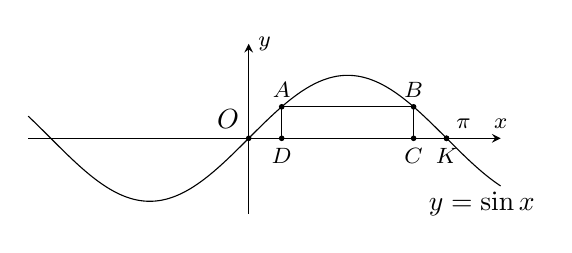
\begin{tikzpicture}[>=stealth,x=1.0cm,y=1.0cm,scale=0.8]
		\draw[->](-3.5,0) --  (4,0) node[above]{\footnotesize $x$};
		\draw[->](0,-1.2) -- (0,1.5)  node[right]{\footnotesize $y$};
		\draw[fill=black] (0,0) node [above left]{$O$} circle (1pt); 
		 \draw[fill=black] (3.14,0) node [above right]{\footnotesize $\pi$} circle (1pt);
		\draw[fill=black] (3.14,0) node [below]{\footnotesize $K$}  circle (1pt);
		\draw[smooth,samples=100,domain=-3.5:4]plot (\x,{sin  ((\x)*180/pi)});
		\draw (pi/6,0)--(pi/6,0.5)--(5*pi/6,0.5)--(5*pi/6,0); 
		\draw[fill=black] (pi/6,0) node [below]{\footnotesize $D$} circle  (1pt);
		\draw[fill=black](pi/6,0.5) node [above]{\footnotesize $A$}  circle (1pt);
		\draw[fill=black] (5*pi/6,0.5) node [above]{\footnotesize  $B$} circle (1pt);
		\draw[fill=black] (5*pi/6,0)  node [below]{\footnotesize $C$} circle (1pt);
		\node at  (3.7,-0.7) [below]{$y=\sin x$};
	\end{tikzpicture}
	} 
	 \loigiai{
		Theo hình vẽ thì $OD=CK \Rightarrow 2OD=\pi-CD=\dfrac{\pi}{3}\Rightarrow OD=\dfrac{\pi}{6}\Rightarrow x_D=\dfrac{\pi}{6}$.\\ 
		Tung độ điểm $D$ là $y_D=\sin\left(\dfrac{\pi}{6} \right)=\dfrac{1}{2}=AD=BC$. 
	} 
\end{ex}

% nguồn: Ok_TraLoiNgan_Lop11_Lan1
\begin{ex}%[1D1V2-3]%[ma:b78ac661]
	Cho tam giác $A B C$, khi đó biểu thức\\ \centerline{$\dfrac{\sin^3\dfrac{B}{2}}{\cos\left(\dfrac{A+C}{2}\right)}+\dfrac{\cos^3\dfrac{B}{2}}{\sin\left(\dfrac{A+C}{2}\right)}-\dfrac{\cos (A+C)}{\sin B}\cdot  \tan B$}\\ bằng?
	 \shortans{2}
	 \loigiai{
		Vì $A+B+C=180^{\circ}$ nên  $A+C=180^{\circ}-B$.\\
		$\begin{aligned}
		\text{VT}& =\dfrac{\sin^3\dfrac{B}{2}}{\cos\left(\dfrac{180^{^\circ}-B}{2}\right)}+\dfrac{\cos^3\dfrac{B}{2}}{\sin\left(\dfrac{180^{^\circ}-B}{2}\right)}-\dfrac{\cos\left(180^\circ-B\right)}{\sin B}\cdot\tan B\\ 
		&=\dfrac{\sin^3\dfrac{B}{2}}{\sin\dfrac{B}{2}}+\dfrac{\cos^3\dfrac{B}{2}}{\cos\dfrac{B}{2}}-\dfrac{-\cos B}{\sin B}\cdot\tan B\\ 
		&=\sin^2\dfrac{B}{2}+\cos^2\dfrac{B}{2}+\cot  B\cdot\tan B=1+1=2=\text{VP}.
\end{aligned}$}
\end{ex}

% nguồn: Ok_TraLoiNgan_Lop11_Lan2
\begin{ex}%[1D1V2-3]%[ma:efe9371f]
	Cho $\tan \alpha+\cot \alpha=m$. Tìm $m$ nguyên dương để $\tan  ^2\alpha+\cot ^2\alpha=7$.
	\shortans{3} 
	\loigiai{ 
		 Ta có $7=\tan ^2\alpha+\cot ^2\alpha=(\tan \alpha+\cot \alpha)^2-2\tan \alpha \cot \alpha=m^2-2$.\\
		Suy ra  $m^2=9\Rightarrow m=3$ (vì $m>0$).
	 }
\end{ex}

% nguồn: Ok_TraLoiNgan_Lop11_Lan2
\begin{ex}%[1D1V2-3]%[ma:07105484]
	Đơn giản các biểu thức sau (giả sử mỗi biểu thức sau luôn có nghĩa)\break $C=\dfrac{\cos ^2x-\sin ^2y}{\sin ^2x \sin ^2y}-\cot  ^2x \cot ^2y$.
	\shortans{-1} 
	 \loigiai{
		\[ 
		\begin{aligned}
			C &=\dfrac{\cos^2 x-\sin^2 y-\cos^2 x \cos^2 y}{\sin^2 x \sin^2 y}=\dfrac{\cos^2 x\left(1-\cos^2 y\right)-\sin^2 y}{\sin^2  x \sin^2 y} \\
			&=\dfrac{\cos^2 x \sin^2 y-\sin^2 y}{\sin^2 x  \sin^2 y}=\dfrac{\sin^2 y\left(\cos^2 x-1\right)}{\sin^2 x \sin^2 y}=\dfrac{-\sin^2 x}{\sin^2 x}=-1
		\end{aligned}
		 \]
	 }
\end{ex}

% nguồn: Ok_TraLoiNgan_Lop11_Lan2
\begin{ex}%[1D1V2-3]%[ma:1610e33a]
	 Biết $\sin a+\cos a=\sqrt{2}$. Tính giá trị của $\sin ^4a+\cos ^4a$.
	 \shortans{0,5}
	\loigiai{ 
		Ta có $\sin  a+\cos a =\sqrt{2}$ \\
		Khi đó $2=(\sin  a+\cos a)^2=\sin^2 a+2 \sin a \cos a+\cos^2 a=1+2 \sin a \cos a$.\\
		Suy ra $\sin a \cos  a=\dfrac{1}{2}$.\\
		Vậy $\sin^4 a+\cos^4 a=\left(\sin ^2a+\cos  ^2a\right)^2-2\sin ^2a \cos ^2a=1-2\left(\dfrac{1}{2}\right)^2=\dfrac{1}{2}=0{,}5$.
	} 
\end{ex}

% nguồn: Ok_TraLoiNgan_Lop11_Lan2
\begin{ex}%[1D1V2-3]%[ma:321c14fa]
	Cho $\tan \alpha=\sqrt{2}$.  Tính giá trị của biểu thức $C=\dfrac{\sin \alpha-\cos \alpha}{\sin ^3\alpha+3\cos ^3\alpha+2\sin \alpha}$. (Kết quả làm tròn đến hàng phần trăm).
	 \shortans{0,08}
	\loigiai{ 
		Vì $\tan \alpha=\sqrt{2}$ nên $\cos \alpha \neq 0$. Chia cả tử và  mẫu của biểu thức $C$ cho $\cos ^3\alpha$, ta được
		 \allowdisplaybreaks
		\begin{eqnarray*}
			C&=&\dfrac{\dfrac{\sin \alpha}{\cos \alpha} \cdot \dfrac{1}{\cos  ^2\alpha}-\dfrac{1}{\cos ^2\alpha}}{\tan ^3\alpha+3+2\cdot \dfrac{\sin \alpha}{\cos \alpha} \cdot \dfrac{1}{\cos ^2\alpha}}\\
			 &=&\dfrac{\tan \alpha\left(1+\tan ^2\alpha\right)-\left(1+\tan ^2\alpha\right)}{\tan ^3\alpha+3+2\tan \alpha\left(1+\tan ^2\alpha\right)}\\
			&=&\dfrac{\left(1+\tan ^2\alpha\right)(\tan \alpha-1)}{3\tan  ^3\alpha+2\tan \alpha+3}\\
			 &=&\dfrac{(1+2)(\sqrt{2}-1)}{3\cdot 2\sqrt{2}+2\sqrt{2}+3}\\
			&=&\dfrac{3(\sqrt{2}-1)}{8\sqrt{2}+3}\approx  0{,}08.
		\end{eqnarray*}
	 }
\end{ex}

% nguồn: Ok_TraLoiNgan_Lop11_Lan1
\begin{ex}%[1D1K2-3]%[ma:b772d384]
	Cho $\tan\alpha+\cot\alpha=m$. Tìm $m>0$ để $\tan  ^2\alpha+\cot ^2\alpha=7$.\\
	\shortans{3} 
	 \loigiai{
		Ta có $7=\tan  ^2\alpha+\cot ^2\alpha=(\tan\alpha+\cot\alpha)^2-2\tan\alpha\cot\alpha=m^2-2$.\\
	Suy ra  $m^2=9\Rightarrow m=3$.}
\end{ex}


%%%%%%%%%%%%%%%% TỰ LUẬN %%%%%%%%%%%%%%%%

% nguồn: Ok_TuanLuan_Toan11_Lan2
\begin{ex}%[1D1H2-3]%[ma:ecc513b2]
	 Cho $\tan x=3$. Tính $P=\dfrac{2\sin x-\cos x}{\sin x+\cos x}$.
	\loigiai{ 
		Ta có $\tan x=3\Rightarrow \dfrac{\sin x}{\cos x}=3\Rightarrow \sin x=3\cos x$.\\ 
		Khi đó $P=\dfrac{2\cdot 3\cos x-\cos x}{3\cos  x+\cos x}=\dfrac{5\cos x}{4\cos x}=\dfrac{5}{4}$.
	} 
\end{ex}

% nguồn: Ok_TuanLuan_Toan11_Lan2
\begin{ex}%[1D1H2-3]%[ma:e38ff563]
	Rút gọn biểu thức $M=\left(\sin x+\cos  x\right)^2+\left(\sin x-\cos x\right)^2$.
	 \loigiai{
		$M=\left(\sin  x+\cos x\right)^2+\left(\sin x-\cos x\right)^2=1+2\sin x\cos x+1-2\sin x\cos x=2.
		 $
	} 
\end{ex}

% nguồn: Ok_TuanLuan_Toan11_Lan2
\begin{ex}%[1D1H2-3]%[ma:16d24767]
	Không dùng máy  tính cầm tay. Hãy tính các giá trị lượng giác sau:
	\begin{listEX}[2]
		\item  $\cos 795^{\circ}$
		\item  $\tan \dfrac{7\pi}{12}$
	\end{listEX}
	\loigiai{ 
		\begin{listEX}
			\item Tính $\cos  795^\circ$.\\
			Vì $795^\circ = 75^\circ + 2 \cdot 360^\circ = 30^\circ + 45^\circ + 2 \cdot 360^\circ$ nên\\ 
			 $\cos 795^\circ = \cos 75^\circ = \cos (30^\circ + 45^\circ) = \cos 30^\circ \cos 45^\circ - \sin 30^\circ \sin 45^\circ = \dfrac{\sqrt{6}-\sqrt{2}}{4}$.
			\item Tính $\tan  \dfrac{7\pi}{12}$.\\
			$\tan \dfrac{7\pi}{12} = \tan \left(\dfrac{\pi}{3} + \dfrac{\pi}{4}\right) = \dfrac{\tan \dfrac{\pi}{3} + \tan \dfrac{\pi}{4}}{1 -  \tan \dfrac{\pi}{3} \tan \dfrac{\pi}{4}} = \dfrac{\sqrt{3} + 1}{1 - \sqrt{3}} = -2 - \sqrt{3}$.\\
		\end{listEX}
	 }
\end{ex}

% nguồn: Ok_TuanLuan_Toan11_Lan2
\begin{ex}%[1D1H2-3]%[ma:32acde94]
	Cho $\sin a=\dfrac{1}{3}$. Tính giá trị của biểu thức $A=\dfrac{\cot a-\tan  a}{\tan a+2\cot a}$.
	 \loigiai{
		Ta có 
		\begin{eqnarray*}
			A&=&\dfrac{\cot a-\tan a}{\tan a+2\cot a}=\dfrac{\dfrac{\cos a}{\sin a}-\dfrac{\sin a}{\cos a}}{\dfrac{\sin  a}{\cos a}+2\dfrac{\cos a}{\sin a}}=\dfrac{\cos ^2a-\sin ^2a}{\sin ^2a+2\cos ^2a}\\
			&=&\dfrac{\left(1-\sin ^2a\right)-\sin ^2a}{\sin ^2a+2\left(1-\sin  ^2a\right)}=\dfrac{1-2\sin ^2a}{2-\sin ^2a}=\dfrac{7}{17}.
		\end{eqnarray*}
	} 
\end{ex}

% nguồn: Ok_TuanLuan_Toan11_Lan2
\begin{ex}%[1D1H2-3]%[ma:a33179c4]
	Cho $\tan \alpha=2$.  Tính giá trị của biểu thức $P=\dfrac{\sin ^4\alpha-3\sin ^3\alpha \cos \alpha+\cos ^2\alpha}{\sin ^2\alpha+\sin ^2\alpha \cos ^2\alpha+2\cos ^2\alpha}$.
	 \loigiai{
		 Do $\tan \alpha=2$ nên $\cos \alpha \neq 0$.\\
		Chia  cả tử và mẫu của biểu thức $P$ cho $\cos ^4\alpha$ ta được
		\begin{eqnarray*}
			P&=&\dfrac{\dfrac{\sin ^4 \alpha}{\cos ^4\alpha}-3 \cdot \dfrac{\sin ^3 \alpha \cos \alpha}{\cos ^4\alpha}+\dfrac{\cos ^2 \alpha}{\cos ^4\alpha}}{\dfrac{\sin ^2 \alpha}{\cos ^4\alpha}+\dfrac{\sin ^2 \alpha \cos ^2 \alpha}{\cos ^4\alpha}+2 \cdot  \dfrac{\cos ^2 \alpha}{\cos ^4\alpha}}\\
			&=&\dfrac{\tan ^4 \alpha-3 \tan ^3 \alpha+\dfrac{1}{\cos ^2 \alpha}}{\tan ^2 \alpha \cdot \dfrac{1}{\cos ^2 \alpha}+\tan ^2 \alpha+2 \cdot  \dfrac{1}{\cos ^2 \alpha}}\\
			&=&\dfrac{\tan ^4 \alpha-3 \tan ^3 \alpha+\left(\tan ^2 \alpha+1\right)}{\tan ^2 \alpha \cdot\left(\tan ^2 \alpha+1\right)+\tan ^2  \alpha+2 \cdot\left(\tan ^2 \alpha+1\right)}\\
			&=&\dfrac{\tan ^4 \alpha-3 \tan ^3 \alpha+\tan ^2 \alpha+1}{\tan ^4 \alpha+4 \tan ^2  \alpha+2} \\
			 &=&\dfrac{2^4-3 \cdot 2^3+2^2+1}{2^4+4 \cdot 2^2+2}\\
			 &=&-\dfrac{3}{34}.
		\end{eqnarray*}
		Vậy $P=-\dfrac{3}{34}$. 
	 }
\end{ex}

% nguồn: Ok_TuanLuan_Toan11_Lan2
\begin{ex}%[1D1H2-3]%[ma:e6a3953f]
	 Cho góc $\alpha$ thỏa mãn $-\dfrac{\pi}{2} < \alpha < 0$ và $\cos \alpha=\dfrac{1}{2}$. Tính trị của biểu thức $P=\sin \alpha+\dfrac{1}{\cos \alpha}$.
	 \loigiai{
		Ta có $\sin ^2\alpha+\cos ^2\alpha=1\Leftrightarrow \sin  ^2\alpha=1-\cos ^2\alpha$.\\
		Với $\cos \alpha=\dfrac{1}{2} \Rightarrow \sin ^2\alpha=1-\left(\dfrac{1}{2}\right)^2=\dfrac{3}{4} \Leftrightarrow \sin \alpha=\pm \dfrac{\sqrt{3}}{2}$.\\ 
		Vì $-\dfrac{\pi}{2} < \alpha < 0$ nên $\sin \alpha < 0\Rightarrow  \sin \alpha=-\dfrac{\sqrt{3}}{2}$.\\
		Vậy  $P=\sin \alpha+\dfrac{1}{\cos \alpha}=-\dfrac{\sqrt{3}}{2}+\dfrac{1}{\dfrac{1}{2}}=-\dfrac{\sqrt{3}}{2}+2=\dfrac{4-\sqrt{3}}{2}$.
	 }
\end{ex}

% nguồn: Ok_TuanLuan_Toan11_Lan2
\begin{ex}%[1D1H2-3]%[ma:0621bee7]
	Thực hiện các yêu cầu trong  các trường hợp sau
	\begin{enumerate}
		\item Tính giá trị lượng giác còn lại  của góc $\alpha$ biết $\sin \alpha=\dfrac{1}{5}$ và $\tan \alpha+\cot \alpha < 0$.
		\item Cho $3\sin  ^4\alpha-\cos ^4\alpha=\dfrac{1}{2}$. Tính $A=2\sin ^4\alpha-\cos ^4\alpha$.
	\end{enumerate}
	\loigiai{ 
		\begin{enumerate}
			\item Ta có $\cot ^2\alpha+1=\dfrac{1}{\sin ^2\alpha}=\dfrac{1}{\left(\dfrac{1}{5} \right)^2}=25\Rightarrow \cot  ^2\alpha=24$ hay $\cot \alpha=\pm 2\sqrt{6}$.\\
			Vì $\tan \alpha$, $\cot \alpha$ cùng dấu và $\tan \alpha+\cot \alpha < 0$ nên $\tan \alpha < 0,\cot \alpha < 0$.\\ 
			Do đó $\cot  \alpha=-2\sqrt{6}$.\\
			Ta lại có $\tan  \alpha=\dfrac{1}{\cot \alpha}=-\dfrac{1}{2\sqrt{6}}$.\\
			Đồng thời, $\cot \alpha=\dfrac{\cos \alpha}{\sin \alpha} \Rightarrow \cos \alpha=\cot \alpha \cdot \sin \alpha=-2\sqrt{6}\cdot  \dfrac{1}{5}=\dfrac{-2\sqrt{6}}{5}$.
			\item  Ta có
			\begin{eqnarray*}
				& &3\sin ^4\alpha-\cos ^4\alpha=\dfrac{1}{2}\\ 
				&\Leftrightarrow& 3\sin ^4\alpha-\left(1-\sin  ^2\alpha \right)^2=\dfrac{1}{2}\\
				&\Leftrightarrow&  6\sin ^4\alpha-2\left(1-2\sin ^2\alpha+\sin ^4\alpha \right)=1\\
				&\Leftrightarrow& 4\sin ^4\alpha+4\sin  ^2\alpha-3=0\\
				&\Leftrightarrow& \left(2\sin ^2\alpha-1\right)\left(2\sin ^2\alpha+3\right)=0\\ 
				&\Leftrightarrow& 2\sin ^2\alpha-1=0. 
			\end{eqnarray*}
			(Do  $2\sin ^2\alpha+3> 0$) suy ra $\sin ^2\alpha=\dfrac{1}{2}$.\\
			Ta lại có $\cos ^2\alpha=1-\sin ^2\alpha=1-\dfrac{1}{2}=\dfrac{1}{2}$  suy ra $A=2\left(\dfrac{1}{2} \right)^2-\left(\dfrac{1}{2} \right)^2=\dfrac{1}{4}$.
	\end{enumerate}}
\end{ex}

% nguồn: Ok_TuanLuan_Toan11_Lan2
\begin{ex}%[1D1H2-3]%[ma:88942c50]
	Chứng  minh các đẳng thức sau
	\begin{enumerate}
		\item $\sin ^4x-\cos ^4x=1-2\cos  ^2x=2\sin ^2x-1$.
		\item $\sin ^3x\cdot \cos x+\sin x\cdot  \cos ^3x=\sin x\cdot \cos x$.
		\item $\tan ^2x-\sin ^2x=\tan ^2x\cdot  \sin ^2x$.
		\item $\cot ^2x-\cos ^2x=\cot ^2x\cdot  \cos ^2x$.
	\end{enumerate}
	\loigiai{ 
		\begin{enumerate}
			\item $\sin ^4x-\cos ^4x$ $=\left(\sin ^2x-\cos ^2x\right)\left(\cos  ^2x+\sin ^2x\right)$ $=-\cos ^2x+\sin ^2x$
			$=-1+\sin ^2x+\sin  ^2x=2\sin ^2x-1=2\left(1-\cos ^2x\right)-1=1-2\cos ^2x
			$. 
			\item $\sin  ^3x\cdot \cos x+\sin x\cdot \cos ^3x=\sin x\cdot \cos x\left(\sin ^2x+\cos ^2x\right)=\sin x\cdot \cos x$
			 \item $\tan ^2x-\sin ^2x=\dfrac{\sin ^2x}{\cos ^2x}-\sin ^2x=\sin ^2x\left(\dfrac{1}{\cos ^2x}-1\right)=\sin ^2x\cdot \dfrac{1-\cos ^2x}{\cos ^2x}=\tan ^2x\cdot \sin ^2x$.
			\item $\cot ^2x-\cos ^2x=\dfrac{\cos ^2x}{\sin^2x}-\cos ^2x=\cos ^2x\left(\dfrac{1}{\sin^2x}-1\right)=\cos ^2x\cdot \dfrac{1-\sin ^2x}{\sin ^2x}=\cot ^2x\cdot  \cos ^2x$.
		\end{enumerate}
	} 
\end{ex}

% nguồn: Ok_TuanLuan_Toan11_Lan2
\begin{ex}%[1D1H2-3]%[ma:a41deb15]
	Chứng minh các đẳng thức  sau
	\begin{enumerate}
		\item $\sin ^4x+\cos  ^4x=1-2\sin ^2x\cdot \cos ^2x$.
		\item $\cos ^4x-\sin  ^4x=\cos ^2x-\sin ^2x$.
		\item $4\cos  ^2x-3=\left(1-2\sin x\right)\left(1+2\sin x\right)$.
		 \item $\left(1+\cos x\right)\left(\sin ^2x-\cos x+\cos ^2x\right)=\sin ^2x$.
	\end{enumerate}
	\loigiai{ 
		\begin{enumerate}
			\item $\sin  ^4x+\cos ^4x=\left(\sin ^2x+\cos ^2x\right)^2-2\sin ^2x\cdot \cos ^2x=1-2\sin ^2x\cdot \cos ^2x$
			\item $\cos ^4x-\sin ^4x=\left(\cos ^2x-\sin  ^2x\right)\left(\cos ^2x+\sin ^2x\right)=\cos ^2x-\sin ^2x$
			\item $\left(1-2\sin  x\right)\left(1+2\sin x\right)=1-4\sin ^2x=1-4\left(1-\cos ^2x\right)=4\cos ^2x-3$
			\item $\left(1+\cos x\right)\left(\sin ^2x-\cos x+\cos  ^2x\right)=\left(1+\cos x\right)\left(1-\cos x\right)=1-\cos ^2x=\sin ^2x$
		\end{enumerate}
	 }
\end{ex}

% nguồn: Ok_TuanLuan_Toan11_Lan2
\begin{ex}%[1D1H2-3]%[ma:5278c84b]
	Chứng minh các đẳng thức sau (giả sử các biểu thức sau đều  có nghĩa)
	\begin{enumerate}
		\item $\cos ^4x+2\sin  ^2x=1+\sin ^4x$.
		\item $\dfrac{\sin x+\cos x}{\sin  ^3x}=\cot ^3x+\cot ^2x+\cot x+1$.
		\item $\dfrac{\cot ^2x-\cot  ^2y}{\cot ^2x\cdot \cot ^2y}=\dfrac{\cos ^2x-\cos ^2y}{\cos ^2x\cdot \cos ^2y}$.
		\item $\sqrt{\sin ^4x+4\cos ^2x}+\sqrt{\cos ^4x+4\sin ^2x}=3\tan \left(x+\dfrac{\pi}{3}  \right)\tan \left(\dfrac{\pi}{6}-x\right)$.
	\end{enumerate}
	 \loigiai{
		\begin{enumerate}
			\item Ta  có
			\begin{align*}
				VT&=\cos ^4x+2\sin  ^2x\\
				&=\left(\cos^2  x\right)^2+2\sin ^2x\\
				&=\left(1-\sin^2x\right)^2+2\sin ^2x\\ 
				&=1-2\sin^2x+\sin^4x+2\sin^2x\\ 
				&=1+\sin^4x=VP. 
			\end{align*}
			 \item Ta có $VT=\dfrac{\sin x+\cos x}{\sin ^3x}=\dfrac{1}{\sin ^2x}+\dfrac{\cos x}{\sin ^3x}$\\
			Mà $\cot ^2x+1=\dfrac{1}{\sin ^2x}$  và $\tan x=\dfrac{\sin x}{\cos x}$ nên
			\[VT=\cot ^2x+1+\cot x\left(\cot  ^2x+1\right)=\cot ^3x+\cot ^2x+\cot x+1=VP.\]
			\item  Ta có
			\begin{align*}
				VT&=\dfrac{\cot ^2x-\cot ^2y}{\cot ^2x\cdot \cot ^2y}\\ 
				&=\dfrac{1}{\cot  ^2y}-\dfrac{1}{\cot ^2x}\\
				&=\tan ^2y-\tan ^2x\\ 
				 &=\left(\dfrac{1}{\cos ^2y}-1\right)-\left(\dfrac{1}{\cos ^2x}-1\right)\\
				&=\dfrac{1}{\cos ^2y}-\dfrac{1}{\cos  ^2x}\\
				&=\dfrac{\cos ^2x-\cos ^2y}{\cos ^2x\cdot \cos  ^2y}=VP.
			\end{align*}
			\item Ta  có
			\begin{align*}
				VT&=\sqrt{\sin ^4x+4\left(1-\sin ^2x\right)}+\sqrt{\cos ^4x+4\left(1-\cos ^2x\right)}\\ 
				&=\sqrt{\left(\sin ^2x\right)^2-4\sin  ^2x+4}+\sqrt{\left(\cos ^2x\right)^2-4\cos ^2x+4}\\
				&=\sqrt{\left(\sin ^2x-2\right)^2}+\sqrt{\left(\cos  ^2x-2\right)^2}\\
				&=\left(2-\sin ^2x\right)+\left(2-\cos  ^2x\right)=4-\left(\sin ^2x+\cos ^2x\right)=3.
			\end{align*}
			 Mặt khác $\left(x+\dfrac{\pi}{3} \right)+\left(\dfrac{\pi}{6}-x\right)=\dfrac{\pi}{2} \Rightarrow \tan \left(\dfrac{\pi}{6}-x\right)=\cot \left(x+\dfrac{\pi}{3} \right)$ nên
			 \[VP=3\tan \left(x+\dfrac{\pi}{3} \right)\cot \left(x+\dfrac{\pi}{3} \right)=3.\]
			 $\Rightarrow VT=VP.$
		\end{enumerate}
	} 
\end{ex}

% nguồn: Ok_TuanLuan_Toan11_Lan2
\begin{ex}%[1D1H2-3]%[ma:04d6f7c9]
	 Biết $\tan \alpha=2$ và $180^{\circ} < \alpha < 270^{\circ}$. Tính giá trị của biểu thức $\sin \alpha+\cos \alpha$
	 \loigiai{
		 Vì $180^{\circ} < \alpha < 270^{\circ}$ nên $\cos \alpha < 0$.\\
		Mà $\cos ^2 \alpha=\dfrac{1}{1+\tan ^2 \alpha}=\dfrac{1}{5} \Rightarrow \cos \alpha=\pm \dfrac{1}{\sqrt{5}}$.\\ 
		Suy ra $\cos  \alpha=-\dfrac{1}{\sqrt{5}}$.\\
		Và $\sin \alpha=\tan \alpha \cdot \cos  \alpha=-\dfrac{2}{\sqrt{5}}$.\\
		Vậy $\sin  \alpha+\cos \alpha=-\dfrac{3\sqrt{5}}{5}$.
	} 
\end{ex}

% nguồn: Ok_TuanLuan_Toan11_Lan2
\begin{ex}%[1D1H2-3]%[ma:e55f0bd4]
	Chứng  minh các đẳng thức sau
	\begin{enumerate}
		\item $\cos  ^2x-\sin ^2x=1-2\sin ^2x$.
		\item $2\cos ^2x-1=1-2\sin ^2x$. 
		\item  $3-4\sin ^2x=4\cos ^2x-1$.
		 \item $\sin x\cot x+\cos x\tan x=\sin x+\cos x$.
	\end{enumerate}
	\loigiai{ 
		\begin{enumerate}
			\item Ta có $\cos  ^2x-\sin ^2x==1-\sin ^2x-\cos ^2x=1-2\sin ^2x$.
			 \item Ta có $2\cos ^2x-1=2\left(1-\sin ^2x\right)-1=1-2\sin ^2x$.
			\item Ta  có $3-4\sin ^2x=3-4\left(1-\cos ^2x\right)=4\cos ^2x-1$.
			\item Ta có $\sin x\cot x+\cos x\tan x=\sin x\cdot \dfrac{\cos x}{\sin x}+\cos x\cdot \dfrac{\sin x}{\cos x}=\sin x+\cos  x$.
		\end{enumerate}
	 }
\end{ex}

% nguồn: Ok_TuanLuan_Toan11_Lan2
\begin{ex}%[1D1H2-3]%[ma:0198a1d3]
	Chứng minh các đẳng thức  sau không phụ thuộc vào biến $x$
	\begin{enumerate}
		 \item $A=-\sin ^4x+\cos ^4x+2\sin ^2x$.
		 \item $B=\sin ^4x+\cos ^2x\sin ^2x+\cos ^2x$.
		\item $B=\cos ^4x+\cos ^2x\sin ^2x+\sin  ^2x$.
	\end{enumerate}
	 \loigiai{
		\begin{enumerate}
			\item Ta có $\begin{aligned}
			-\sin ^4x+\cos ^4x+2\sin ^2x&=\left(\sin ^2x-\cos ^2x\right)\left(\sin ^2x+\cos ^2x\right)+2\sin ^2x\\ 
			 &=\sin ^2x+\cos ^2x=1.
		\end{aligned}$
		\item Ta có $\begin{aligned}
		B=&\sin ^4x+\cos ^2x\sin  ^2x+\cos ^2x=\sin ^2x\left(\sin ^2x+\cos ^2x\right)+\cos ^2x\\
		=&\sin ^2x+\cos ^2x=1. 
	\end{aligned}$
	\item Ta có $B=\cos ^4x+\cos ^2x\sin ^2x+\sin ^2x=\cos ^2x\left(\cos ^2x+\sin  ^2x\right)+\sin ^2x =\cos ^2x + \sin ^2x=1$.
	\end{enumerate}
} 
\end{ex}

% nguồn: Ok_TuanLuan_Toan11_Lan2
\begin{ex}%[1D1H2-3]%[ma:f1c6b926]
	Chứng  minh biểu thức sau không phụ thuộc vào $x$.
	\begin{enumerate}
		\item $A=\dfrac{\sin ^6x+\cos ^6x+2}{\sin ^4x+\cos  ^4x+1}$.
		\item  $B=\dfrac{1+\cot x}{1-\cot x}-\dfrac{2+2\cot ^2x}{\left(\tan x-1\right)\left(\tan ^2x+1\right)}$.
		\item $C=\sqrt{\sin ^4x+6\cos ^2x+3\cos  ^4x}+\sqrt{\cos ^4x+6\sin ^2x+3\sin ^4x}$.
	\end{enumerate}
	 \loigiai{
		\begin{enumerate}
			\item Ta  có
			\begin{itemize}
				\item $\sin ^4\alpha+\cos ^4\alpha=\left(\sin ^2\alpha+\cos ^2\alpha \right)^2-2\sin ^2\alpha  \cos ^2\alpha=1-2\sin ^2\alpha \cos ^2\alpha$.
				 \item
				\begin{align*}
					\sin ^6\alpha+\cos ^6\alpha&=\left(\sin ^2\alpha  \right)^3+\left(\cos ^2\alpha \right)^3\\
					&=\left(\sin ^2\alpha+\cos ^2\alpha \right)\left(\sin  ^4\alpha+\cos ^4\alpha-\sin ^2\alpha \cos ^2\alpha \right)\\
					&=\sin  ^4\alpha+\cos ^4\alpha-\sin ^2\alpha \cos ^2\alpha\\
					&=1-2\sin ^2\alpha \cos ^2\alpha-\sin ^2\alpha \cos ^2\alpha=1-3\sin ^2\alpha \cos  ^2\alpha.
				\end{align*}
			\end{itemize}
			Do đó $A=\dfrac{1-3\sin ^2\alpha \cos  ^2\alpha+2}{1-2\sin ^2\alpha \cos ^2\alpha+1}=\dfrac{3\left(1-\sin ^2\alpha \cos ^2\alpha \right)}{2\left(1-\sin ^2\alpha \cos ^2\alpha \right)}=\dfrac{3}{2}$.\\
			Vậy $A$ không phụ  thuộc vào $x$.
			 \item Ta có
			\begin{align*}
				B&=\dfrac{1+\dfrac{1}{\tan x}}{1-\dfrac{1}{\tan x}}-\dfrac{2+\dfrac{2\cos  ^2x}{\sin ^2x}}{\left(\tan x-1\right)\dfrac{1}{\sin ^2x}}\\
				&=\dfrac{\tan x+1}{\tan x-1}-\dfrac{2\left(\sin  ^2x+\cos ^2x\right)}{\tan x-1}\\
				&=\dfrac{\tan x+1-2}{\tan  x-1}=1.
			\end{align*}
			 Vậy $B$ không phụ thuộc vào $x$.
			\item Ta có 
			\begin{align*}
				C&=\sqrt{\left(1-\cos ^2x\right)^2+6\cos ^2x+3\cos ^4x}+\sqrt{\left(1-\sin  ^2x\right)^2+6\sin ^2x+3\sin ^4x}\\
				&=\sqrt{4\cos ^4x+4\cos  ^2x+1}+\sqrt{4\sin ^4x+4\sin ^2x+1}\\
				&=\sqrt{\left(2\cos  ^2x+1\right)^2}+\sqrt{\left(2\sin ^2x+1\right)^2}\\
				&=2\cos ^2x+1+2\sin  ^2x+1=4.
			\end{align*}
			Vậy $C$ không phụ thuộc  vào $x$.
		\end{enumerate}
	 }
\end{ex}

% nguồn: Ok_TuanLuan_Toan11_Lan2
\begin{ex}%[1D1H2-3]%[ma:e281647e]
	Đơn  giản biểu thức $A=\dfrac{\left(\sin x-\cos x\right)^2-1}{\tan x-\sin x\cdot \cos x}$.
	\loigiai{ 
		Ta có 
		\[A=\dfrac{\left(\sin x-\cos x\right)^2-1}{\tan x-\sin x\cdot \cos x}=\dfrac{-2\cos x\cdot \sin x}{\dfrac{\sin x}{\cos x}-\sin x\cdot \cos x}=\dfrac{-2\cos x\cdot \sin x\cos x}{\sin x\left(1-\cos ^2x\right)}=\dfrac{-2\cos  ^2x}{\sin ^2x}=-2\cot ^2x.\]
	 }
\end{ex}

% nguồn: Ok_TuanLuan_Toan11_Lan2
\begin{ex}%[1D1H2-3]%[ma:c4f2b6e5]
	 Rút gọn các biểu thức sau
	\begin{enumerate}
		 \item $\sin ^2\left(3\pi-\alpha \right)+\sin ^2\left(\alpha+\dfrac{5\pi}{2} \right)$.
		\item $\left[1+\tan ^2\left(-\alpha+11\pi \right)\right]\cdot \sin  ^2\left(\alpha-\dfrac{3\pi}{2} \right)$.
	\end{enumerate}
	\loigiai{ 
		\begin{enumerate}
			\item Ta có 
			\begin{itemize}
				\item $\sin  \left(3\pi-\alpha \right)=\sin \left(\pi-\alpha+2\pi \right)=\sin \left(\pi-\alpha \right)=\sin \alpha$.
				\item $\sin \left(\alpha+\dfrac{5\pi}{2} \right)=\sin \left(\alpha+\dfrac{\pi}{2}+2\pi \right)=\sin \left(\alpha+\dfrac{\pi}{2} \right)=\cos \left(-\alpha \right)=\cos  \alpha.$
			\end{itemize}
			Suy ra, $\sin ^2\left(3\pi-\alpha \right)+\sin ^2\left(\alpha+\dfrac{5\pi}{2} \right)=\sin ^2\alpha+\cos ^2\alpha=1$. 
			 \item Ta có
			\begin{itemize}
				\item $\tan \left(-\alpha+11\pi \right)=\tan \left(-\alpha  \right)=-\tan \alpha$.
				\item $\sin \left(\alpha-\dfrac{3\pi}{2} \right)=\sin \left(\alpha+\dfrac{\pi}{2}-2\pi \right)=\sin \left(\alpha+\dfrac{\pi}{2} \right)=\cos \left(-\alpha  \right)=\cos \alpha$.
			\end{itemize}
			Suy ra, $\left[1+\tan ^2\left(-\alpha+11\pi \right)\right].\sin ^2\left(\alpha-\dfrac{3\pi}{2} \right)=\left(1+\tan ^2\alpha \right)\cdot  \cos ^2\alpha$ $=\dfrac{1}{\cos ^2\alpha}\cdot \cos ^2\alpha=1$.
		\end{enumerate}
	} 
\end{ex}

% nguồn: Ok_TuanLuan_Toan11_Lan2
\begin{ex}%[1D1H2-3]%[ma:9194d73d]
	Cho $\tan \alpha=3$, tính giá trị của biểu  thức $P=\dfrac{2\sin \alpha-\cos \alpha}{3\sin \alpha-5\cos \alpha}$.
	\loigiai{ 
		Chia cả tử và mẫu của $P$ cho $\cos \alpha  \neq 0$ ta được
		\[P=\dfrac{2\sin \alpha-\cos \alpha}{3\sin \alpha-5\cos \alpha}=\dfrac{2\tan \alpha-1}{3\tan \alpha-5}=\dfrac{5}{4}.\] 
	 }
\end{ex}

% nguồn: Ok_TuanLuan_Toan11_Lan2
\begin{ex}%[1D1H2-3]%[ma:944a18d4]
	Cho  $\sin x+\cos x=m$. Tính giá trị của biểu thức $M=|\sin x-\cos x|$.
	\loigiai{ 
		Ta có $M^2=(\sin x-\cos x)^2=\sin ^2x-2\sin x \cdot \cos x+\cos ^2x=1-2\sin x \cdot \cos  x$.\\
		Mặt khác $M^2=(\sin x-\cos x)^2=(\sin x+\cos x)^2-4\sin x \cdot \cos x=m^2-4\sin x  \cdot \cos x$.\\
		Suy ra $1-2\sin x \cdot \cos x=m^2-4\sin x \cdot \cos x  \Leftrightarrow \sin x \cdot \cos x=\dfrac{m^2-1}{2}$.\\
		Do  đó $M^2=2-m^2\Rightarrow M=\sqrt{2-m^2}$.
	} 
\end{ex}

% nguồn: Ok_TuanLuan_Toan11_Lan2
\begin{ex}%[1D1H2-3]%[ma:6dbe7cbd]
	Rút gọn các biểu  thức sau:
	\begin{listEX}
		\item $A  = \sin (x+14^\circ) \sin (x+74^\circ) + \sin (x-76^\circ) \sin (x-16^\circ)$.
		\item $B = \dfrac{\sin (a-b)}{\cos a \cos b} + \dfrac{\sin (b-c)}{\cos  b \cos c} + \dfrac{\sin (c-a)}{\cos c \cos a}$.
	\end{listEX}
	 \loigiai{
		\begin{listEX}
			\item Ta có $A =  \sin(14^\circ + x)\cos(16^\circ - x) + \sin(76^\circ - x)\sin(16^\circ - x)$\\
			$=  \sin(14^\circ + x)\cos(16^\circ - x) + \cos(14^\circ + x)\sin(16^\circ - x)$.
			$= \sin(14^\circ + x + 16^\circ  - x) = \sin 30^\circ = \dfrac{1}{2}$.
			\item  $B = \dfrac{\sin (a-b)}{\cos a \cos b} + \dfrac{\sin (b-c)}{\cos b \cos c} + \dfrac{\sin (c-a)}{\cos c \cos a}$.\\
			Ta có $B = \dfrac{\sin a \cos b - \sin b \cos a}{\cos a \cos b} + \dfrac{\sin b \cos c - \sin c \cos b}{\cos b \cos c} + \dfrac{\sin c \cos a  - \sin a \cos c}{\cos c \cos a}$.\\
			$= \dfrac{\sin a \cos b}{\cos a \cos b} - \dfrac{\sin b \cos a}{\cos a \cos b} + \dfrac{\sin b \cos c}{\cos b \cos c} - \dfrac{\sin c \cos b}{\cos b  \cos c} + \dfrac{\sin c \cos a}{\cos c \cos a} - \dfrac{\sin a \cos c}{\cos c \cos a}$.\\
			$= \tan a - \tan b + \tan b - \tan c + \tan c  - \tan a = 0$.
		\end{listEX}
	} 
\end{ex}

% nguồn: Ok_TuanLuan_Toan11_Lan2
\begin{ex}%[1D1H2-3]%[ma:dc4b050f]
	Rút gọn biểu thức $A=\left(1-\sin ^2x\right)\cdot \cot ^2x+\left(1-\cot ^2x\right)$. 
	 \loigiai{
		$A=\left(1-\sin  ^2x\right)\cdot \cot ^2x+\left(1-\cot ^2x\right)=\cot ^2x-\cos ^2x+1-\cot ^2x=\sin ^2x
		 $.
	 }
\end{ex}

% nguồn: Ok_TuanLuan_Toan11_Lan2
\begin{ex}%[1D1H2-3]%[ma:04d277d6]
	 Cho $\tan x=-4$. Giá trị của biểu thức $A=\dfrac{2\sin x-5\cos x}{3\cos x+\sin x}$ là
	\loigiai{ 
		Chia cả tử  và mẫu của $A$ cho $\cos x \neq 0$ ta được
		\[A=\dfrac{2\sin x-5\cos x}{3\cos x+\sin x}=\dfrac{2\dfrac{\sin x}{\cos x}-5\dfrac{\cos x}{\cos x}}{3\dfrac{\cos x}{\cos x}+\dfrac{\sin x}{\cos  x}}=\dfrac{2\tan x-5}{3+\tan x}=\dfrac{2\cdot(-4)-5}{3+(-4)}=13.\]
	} 
\end{ex}

% nguồn: Ok_TuanLuan_Toan11_Lan2
\begin{ex}%[1D1H2-3]%[ma:af02be39]
	Tính giá  trị của biểu thức $A=\sin ^6\alpha+\cos ^6\alpha+3\sin ^2\alpha \cos ^2\alpha$.
	\loigiai{ 
		Ta  có
		 $\sin ^6\alpha+\cos ^6\alpha=\left(\sin ^2\alpha+\cos ^2\alpha \right)^2-3\sin ^2\alpha \cos ^2\alpha \left(\sin ^2\alpha+\cos ^2\alpha \right)=1-3\sin ^2\alpha \cos ^2\alpha.
		 $\\
		Suy ra $A=1-3\sin  ^2\alpha \cos ^2\alpha+3\sin ^2\alpha \cos ^2\alpha=1$.
	 }
\end{ex}

% nguồn: Ok_TuanLuan_Toan11_Lan2
\begin{ex}%[1D1H2-3]%[ma:69bdbcff]
	Chứng minh các  đẳng thức lượng giác sau
	\begin{enumerate}
		\item $\dfrac{\sin ^3\alpha+\cos ^3\alpha}{\sin \alpha+\cos  \alpha}=1-\sin \alpha \cos \alpha$.
		\item  $\dfrac{1+\tan \alpha}{1-\tan \alpha}+\dfrac{1+\cot \alpha}{1-\cot \alpha}=0$.
	\end{enumerate}
	\loigiai{ 
		\begin{enumerate}
			\item 
			\begin{align*}
				\dfrac{\sin ^3\alpha+\cos ^3\alpha}{\sin \alpha+\cos \alpha}&=\dfrac{\left(\sin \alpha+\cos \alpha \right)\cdot \left(\sin ^2\alpha-\sin \alpha \cos \alpha+\cos ^2\alpha \right)}{\sin \alpha+\cos  \alpha}\\
				&=\sin ^2\alpha-\sin \alpha \cos \alpha+\cos ^2\alpha=1-\sin  \alpha \cos \alpha.
			\end{align*}
			\item 
			\begin{align*}
				\dfrac{1+\tan \alpha}{1-\tan \alpha}+\dfrac{1+\cot \alpha}{1-\cot \alpha}&=\dfrac{\tan \alpha \cdot \cot \alpha+\tan \alpha}{\tan \alpha \cdot \cot \alpha-\tan \alpha}+\dfrac{1+\cot \alpha}{1-\cot \alpha}\\ 
				&=\dfrac{\tan \alpha \left(\cot \alpha+1\right)}{\tan \alpha \left(\cot  \alpha-1\right)}+\dfrac{1+\cot \alpha}{1-\cot \alpha}\\
				&=\dfrac{\cot \alpha+1}{\cot  \alpha-1}-\dfrac{1+\cot \alpha}{\cot \alpha-1}=0.
			\end{align*}
	\end{enumerate}}
\end{ex}

% nguồn: Ok_TuanLuan_Toan11_Lan2
\begin{ex}%[1D1H2-3]%[ma:df69ee64]
	Tính giá  trị của các biểu thức sau đây
	\begin{enumerate}
		\item $A=\sin ^25^{\circ}+\sin  ^210^{\circ}+\sin ^215^{\circ}+\cdots+\sin ^285^{\circ}$ (17 số hạng).
		\item $B=\cos 5^{\circ}+\cos 10^{\circ}+\cos 15^{\circ}+\cdots+\cos  175^{\circ}$ (35 số hạng)
	\end{enumerate}
	 \loigiai{
		\begin{enumerate}
			\item Vận dụng $\sin \left(90^{\circ}-\alpha \right)=\cos  \alpha$.\\
			 Ta có
			\begin{itemize}
				\item $\sin 85^{\circ}=\cos 5^{\circ}$. 
				\item  $\sin 80^{\circ}=\cos 10^{\circ}$.
				\item  $\sin 75^{\circ}=\cos 15^{\circ}$.
				\item  $\ldots$
				 \item $\sin 50^{\circ}=\cos 40^{\circ}$.
			\end{itemize}
			 Vậy
			\begin{align*}
				A&=\left(\sin ^25^{\circ}+\cos ^25^{\circ}  \right)+\left(\sin ^210^{\circ}+\cos ^210^{\circ} \right)+\cdots+\left(\sin ^240^{\circ}+\cos ^240^{\circ} \right)+\sin ^245^{\circ}\\
				&=\underbrace{1+1+\cdots+1}_{\text{8  số 1}}+\left(\dfrac{\sqrt{2}}{2} \right)^2=\dfrac{17}{2}.
			\end{align*}
			\item Vận  dụng $\cos \left(180^{\circ}-\alpha \right)=-\cos \alpha$.\\
			Ta  có
			\begin{itemize}
				\item $\cos 175^{\circ}=-\cos 5^{\circ}$. 
				\item $\cos 170^{\circ}=-\cos  10^{\circ}$.
				\item $\cos165^{\circ}=-\cos  15^{\circ}$.
				\item  $\ldots$
				\item $\cos 95^{\circ}=-\cos 85^{\circ}$. 
			\end{itemize}
			Vậy 
			\begin{align*}
				B&=\left(\cos 5^{\circ}+\cos  175^{\circ} \right)+\left(\cos 10^{\circ}+\cos 170^{\circ} \right)+\cdots+\left(\cos 85^{\circ}+\cos 95^{\circ} \right)+\cos 90^{\circ}\\
				 &=\underbrace{0+0+\cdots+0}_{\text{17 số 1}}+\cos 90^{\circ}=0.
			\end{align*}
	\end{enumerate}}
\end{ex}

% nguồn: Ok_TuanLuan_Toan11_Lan2
\begin{ex}%[1D1H2-3]%[ma:ba157c28]
	Cho $\tan \alpha=2$. Tính giá trị của  biểu thức: $A=\dfrac{3\sin \alpha+\cos \alpha}{\sin \alpha-\cos \alpha}$
	\loigiai{ 
		Chia cả tử và mẫu của  $A$ cho $\cos \alpha \neq 0$ ta được
		\[A=\dfrac{3\sin \alpha+\cos \alpha}{\sin  \alpha-\cos \alpha}=\dfrac{3 \tan \alpha+1}{\tan \alpha-1}=7.\]
	 }
\end{ex}

% nguồn: Ok_TuanLuan_Toan11_Lan2
\begin{ex}%[1D1V2-3]%[ma:21409d1c]
	Rút gọn biểu thức $C=2\left(\cos ^4x+\sin ^4x+\cos ^2x\sin  ^2x\right)^2-\left(\cos ^8x+\sin ^8x\right)$.
	 \loigiai{
		 Ta có
		\begin{eqnarray*}
			\cos ^8x+\sin ^8x &=&\left(\cos ^2x+\sin ^2x\right)^2-2\cos ^2x\sin  ^2x=1-2\cos ^2x\sin ^2x \\
			&= &\left(\cos  ^4x+\sin ^4x\right)^2-2\cos ^4x\sin ^4x= 1-4\cos ^2x\sin ^2x+2\cos ^4x\sin ^4x\\
			&=&\left(1-2\cos ^2x\sin ^2x\right)^2-2\cos ^4x\sin ^4x = 1-4\cos ^2x\sin ^2x+2\cos ^4x\sin  ^4x.
		\end{eqnarray*}
		Suy ra 
		\begin{eqnarray*}
			C&=&2\left(1-\cos ^2x\sin ^2x\right)^2-\left(1-4\cos ^2x\sin ^2x+2\cos ^4x\sin  ^4x\right)\\
			&=&2\left(1-2\cos ^2x\sin ^2x+\cos ^4x\sin  ^4x\right)-\left(1-4\cos ^2x\sin ^2x+2\cos ^4x\sin ^4x\right) = 1.
		\end{eqnarray*}
		 Vậy $C=1$.
	 }
\end{ex}

% nguồn: Ok_TuanLuan_Toan11_Lan2
\begin{ex}%[1D1V2-3]%[ma:53e3a428]
	 Cho $0< \alpha < \dfrac{\pi}{2}$. Tính $\sqrt{\dfrac{1+\sin \alpha}{1-\sin \alpha}}+\sqrt{\dfrac{1-\sin \alpha}{1+\sin \alpha}}$.
	 \loigiai{
		Đặt  $A=\sqrt{\dfrac{1+\sin \alpha}{1-\sin \alpha}}+\sqrt{\dfrac{1-\sin \alpha}{1+\sin \alpha}}$\\
		Khi đó $A^2=\left(\sqrt{\dfrac{1+\sin \alpha}{1-\sin \alpha}}+\sqrt{\dfrac{1-\sin \alpha}{1+\sin \alpha}} \right)^2=\dfrac{1+\sin \alpha}{1-\sin \alpha}+\dfrac{1-\sin  \alpha}{1+\sin \alpha}+2=\dfrac{4}{\cos ^2\alpha}$.\\
		Vì $0< \alpha < \dfrac{\pi}{2}$ nên $\cos \alpha > 0$  do đó $A=\dfrac{2}{\cos \alpha}$.
	 }
\end{ex}

% nguồn: Ok_TuanLuan_Toan11_Lan2
\begin{ex}%[1D1V2-3]%[ma:afd8142f]
	Chứng minh  các đẳng thức sau
	\begin{enumerate}
		\item $\tan x+\cot  x=\dfrac{1}{\sin x\cdot \cos x}$.
		\item $\dfrac{1-\cos x}{\sin x}=\dfrac{\sin  x}{1+\cos x}$.
		\item $\dfrac{1}{1+\tan  x}+\dfrac{1}{1+\cot x}=1$.
		\item $\left(1-\dfrac{1}{\cos x}  \right)\left(1+\dfrac{1}{\cos x} \right)+\tan ^2x=0$.
	\end{enumerate}
	 \loigiai{
		\begin{enumerate}
			\item $\tan x+\cot x=\dfrac{\sin x}{\cos x}+\dfrac{\cos x}{\sin x}=\dfrac{\sin ^2x+\cos ^2x}{\sin x\cdot  \cos x}=\dfrac{1}{\sin x\cdot \cos x}$.
			\item $\begin{aligned}
			\dfrac{1-\cos x}{\sin x}=\dfrac{\sin x}{1+\cos  x} &\Leftrightarrow \left(1-\cos x\right)\left(1+\cos x\right)=\sin ^2x\\
			&\Leftrightarrow 1-\cos ^2x=\sin  ^2x\\
			&\Leftrightarrow \sin  ^2x+\cos ^2x=1
		\end{aligned}$
		\item $\dfrac{1}{1+\tan x}+\dfrac{1}{1+\cot x}=\dfrac{1}{1+\tan x}+\dfrac{1}{1+\dfrac{1}{\tan x}}=\dfrac{1}{1+\tan x}+\dfrac{\tan x}{1+\tan  x}=1$.
		\item $\left(1-\dfrac{1}{\cos x} \right)\left(1+\dfrac{1}{\cos x} \right)+\tan ^2x=1-\dfrac{1}{\cos ^2x}+\dfrac{\sin ^2x}{\cos ^2x}=\dfrac{\sin ^2x+\cos  ^2x-1}{\cos ^2x}=0$.
	\end{enumerate}
} 
\end{ex}
